\documentclass[12pt]{article}
\usepackage{geometry}
\usepackage{hyperref}
\usepackage{graphicx}
\usepackage{titlesec}
\usepackage{fancyhdr}
\usepackage{float}
\usepackage[all]{hypcap}


% 设置页边距
\geometry{a4paper, left=25mm, right=25mm, top=30mm, bottom=30mm}

% 修复 fancyhdr 警告
\setlength{\headheight}{14.49998pt}

% 页眉页脚设置
\pagestyle{fancy}
\fancyhf{}
\fancyhead[L]{COMP3019J University Website Project}
\fancyhead[R]{\thepage}
\fancyfoot[L]{Group 20}
\fancyfoot[R]{October, 2024}

% 标题格式设置
\titleformat{\section}
  {\large\bfseries}{\thesection}{1em}{}
\titleformat{\subsection}
  {\normalsize\bfseries}{\thesubsection}{1em}{}

% 生成可点击链接
\hypersetup{
    colorlinks=true,
    linkcolor=blue,
    filecolor=magenta,      
    urlcolor=cyan,
    pdftitle={COMP 3019J Project},
    pdfpagemode=FullScreen,
}

% 文档标题
\title{COMP3019J University Website Project\\ \Large Design Document}
\date{October 2024}

\begin{document}

% 第一页:标题页
\maketitle
\vspace{2cm}
\begin{figure}[h]  % 插入图片的部分
  \centering
  
\includegraphics[width=0.8\textwidth]{title.png}  % 替换成你的图片文件名
\end{figure}

\vspace{4cm}

% 插入作者和日期信息作为文本
\begin{center}
  \textbf{Bohan Zhang 22207251}\\
  \textbf{Yunhan Gao 22207250}\\
  \textbf{Le Liu 22207256}\\
  \vspace{0.5cm}  % 添加一点间距以分隔信息
  \textbf{Group  20}\\  % 替换成你的组号
  \vspace{0.5cm}

\end{center}

\thispagestyle{empty}
\newpage

% 第二页:目录页
\tableofcontents
\newpage

% 开始正文

\section{Introduction}

\subsection{Project Goals}
The primary goal of this project is to design and implement a comprehensive university website that offers a personalized
 and functional experience for different types of users. The website will provide students, teachers, library staff and other security personnel with an interface to manage their profiles, interact with others, and access university resources based on their 
 roles. The website is expected to enhance user engagement, facilitate communication, and streamline administrative processes 
 within the university. 

\subsection{Target Users and Use Cases} The target users of the website include students, teachers, library staff, security personnel, 
administrative staff and external visitors. Each user type has specific features tailored to their role:

\begin{itemize}
  \item \textbf{Students}: Students will have access to their dashboard, which display timetables, profiles, and 
  enrolled courses. They can register for courses, check their grades, interact with teachers and fellow students, view library 
  collections, and check their own borrowing history, as well as manage their electric bike licenses.
  \item \textbf{Teachers}: Teachers will have a dashboard that shows the courses they teach, timetable, profiles, and office 
  location. They can create and manage courses, interact with students, view library collections.
  \item \textbf{Library staff}: Library staff will have access to features that allow them to manage book inventories, track book 
  loans, and assist users with book reservations. They can also update library resources and monitor the availability of digital 
  content for users.
  \item \textbf{Security personnel}: Security personnel will manage electric bike licenses and oversee vehicle registrations on 
  campus.
  \item \textbf{Administrative staff}: Administrative users will have full control over the system, including managing user 
  registrations, overseeing course creation, and handling overall database management to ensure smooth system operation.
  \item \textbf{External visitors}: Unregistered users will have limited access to parts of the website, such as viewing general 
  information about the university, available library resources without the ability  interact with internal functions.  
\end{itemize}

\subsection{Technological Stack Overview}
The university website will be built using a modern and robust technological stack to ensure reliability, security, and scalability. 
The core technologies to be used include:
\begin{itemize}
    \item \textbf{Frontend}: The user interface will be developed using HTML, CSS, and JavaScript to create an interactive and
     responsive design. Libraries like Bootstrap or Material UI may be incorporated for consistent styling across the website.
    \item \textbf{Backend}: The server-side logic will be implemented using Flask (Python), providing a flexible framework for 
    managing user authentication, database interactions, and session management.
    \item \textbf{Database}: MySQL will be used as the primary database management system to store user profiles, 
    course data, library resources, electric bike licenses, and forum information. The database will include the design of 
    tables with appropriate relationships, such as primary and foreign keys, to ensure data integrity and support efficient 
    querying and management.
    \item \textbf{Security}: The website will ensure secure handling of sensitive data, such as passwords, using encryption 
    mechanisms. Proper user authentication and authorization will be implemented to protect user privacy and data access.
\end{itemize}
This technology stack has been chosen for its simplicity, flexibility, and suitability for the scale of the university website project, 
ensuring a smooth user experience and maintainability.

\newpage
\section{Website Functionalities}
\subsection{System Use Case Overview}

The following sections describe the system's functionalities. The \textit{Common Use Cases} subsection outlines features accessible to multiple user types, such as library search and forum participation. Subsequent sections cover features unique to each user type, including course management for teachers and e-bike management for security personnel.\\ \\ 
The Use Case Diagram is below:

\begin{figure}[h]
    \centering
    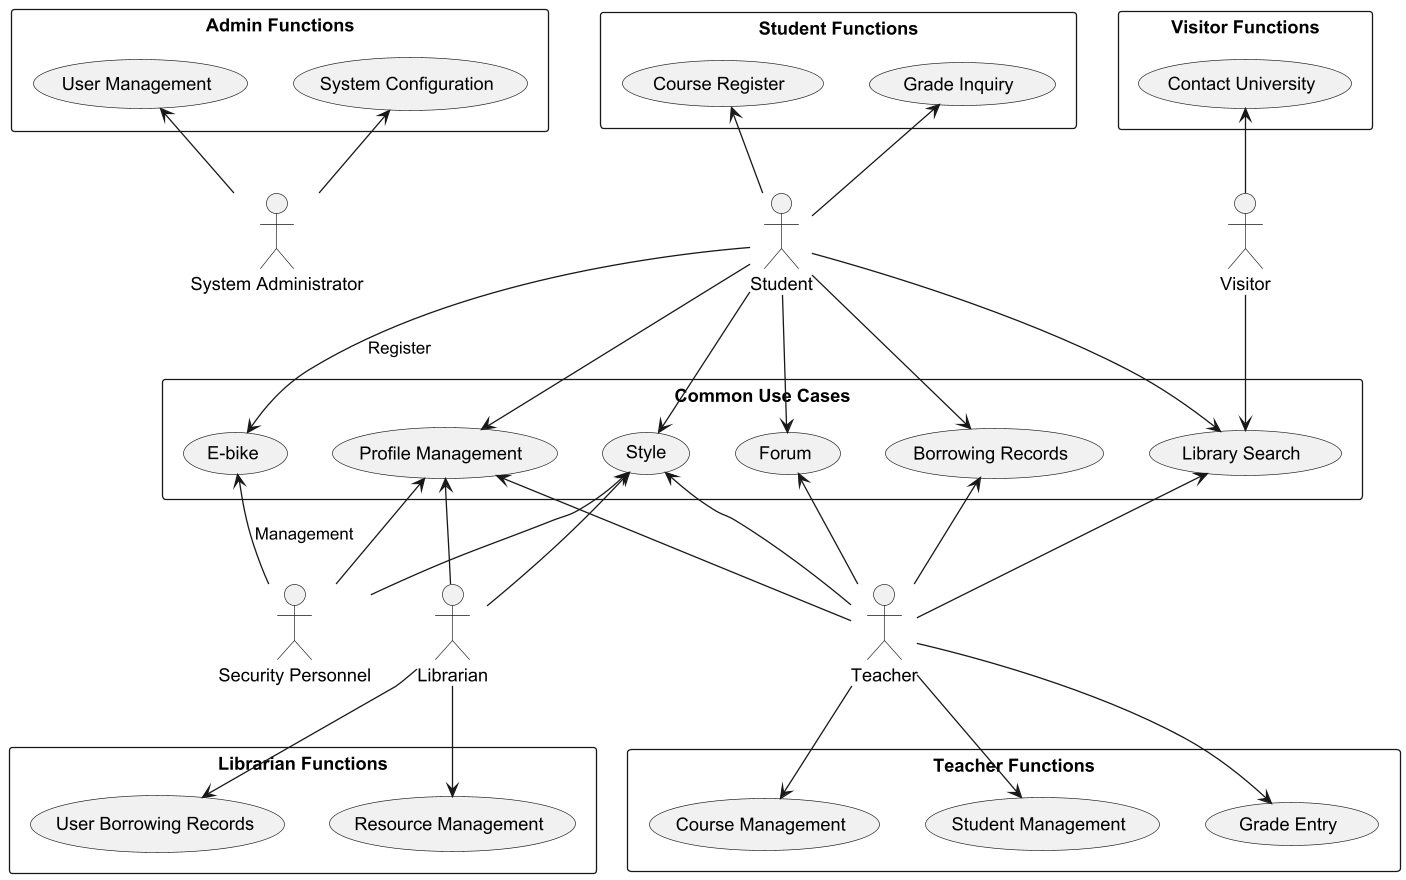
\includegraphics[width=0.8\textwidth]{usecasediagram.png}  % 替换成你的图片文件名
    \caption{System Use Case Diagram}
    \label{fig:use_case_diagram}
\end{figure}

\subsection{Common Use Cases}
\subsubsection{Library Search}

\paragraph{Description}
The Library Search allows students, teachers, and visitors to search for books, journals, and articles using various criteria like title, author, or keywords. Logged-in users can also view their borrowing history. After using this feature, users obtain detailed information about resource availability and location.
\paragraph{Data Outcomes}
\begin{itemize}
    \item \textbf{READ} - Library resource information, availability status, resource location
    \item \textbf{CREATE} - Search history log entry (for logged-in users)
\end{itemize}

\paragraph{Related UI}
For the related user interface, click \hyperref[fig:searchbook_page]{Figure~\ref*{fig:searchbook_page}}.

\subsubsection{Borrowing Records}

\paragraph{Description}
Borrowing Records enables students and teachers to view their current loans, due dates, past borrowing history, and any overdue fines. Users can also renew eligible items. After using this feature, users can track their borrowed items and manage renewals.

\paragraph{Data Outcomes}
\begin{itemize}
    \item \textbf{READ} - Current borrowed items, due dates, past borrowing history, fines/penalties
    \item \textbf{UPDATE} - Loan status and due dates (in case of renewals)
    \item \textbf{CREATE} - Log entry of borrowing record access
\end{itemize}

\paragraph{Related UI}
For the related user interface, click \hyperref[fig:loanrecord_page]{Figure~\ref*{fig:loanrecord_page}}.

\subsubsection{Profile Management}

\paragraph{Description}
Profile Management allows students, teachers, librarians, and security personnel to update personal information such as contact details, privacy settings, and profile pictures. After using this feature, users will have updated their profile with any necessary changes reflected in the system.

\paragraph{Data Outcomes}
\begin{itemize}
    \item \textbf{READ} - Current profile information
    \item \textbf{UPDATE} - Personal details, contact information, privacy settings
    \item \textbf{CREATE} - Log entry of profile changes
\end{itemize}

\paragraph{Related UI}
For the related user interface, click \hyperref[fig:student_profile_page]{Figure~\ref*{fig:student_profile_page}}.

\subsubsection{Forum Participation}

\paragraph{Description}
Forum Participation allows students and teachers to create or reply to discussion threads on various academic or campus-related topics. After using this feature, users contribute to ongoing discussions or start new ones to engage with the university community.

\paragraph{Data Outcomes}
\begin{itemize}
    \item \textbf{CREATE} - New forum posts or replies
    \item \textbf{READ} - Existing forum threads and replies
    \item \textbf{UPDATE} - User's forum activity status
\end{itemize}

\paragraph{Related UI}
For the related user interface, click \hyperref[fig:forum_page]{Figure~\ref*{fig:forum_page}}.

\subsubsection{Style Customization}

\paragraph{Description}
Style Customization enables students, teachers, librarians, and security personnel to personalize the interface by adjusting settings such as color schemes and fonts. After using this feature, users will have their preferred visual settings applied, improving their experience.

\paragraph{Data Outcomes}
\begin{itemize}
    \item \textbf{READ} - Current style settings
    \item \textbf{UPDATE} - User's style preferences
    \item \textbf{CREATE} - Log entry of style changes
\end{itemize}

\subsection{Student Functions}
\subsubsection{Course Register}

\paragraph{Description}
The Course Register feature allows students to view available courses, register for classes, and drop courses during specified periods. After using this feature, students can view their updated course schedule, along with confirmation of their successful registrations or drops.

\paragraph{Data Outcomes}
\begin{itemize}
    \item \textbf{READ} - Available courses, current course schedule, course details
    \item \textbf{CREATE} - New course registrations
    \item \textbf{UPDATE} - Student's course schedule
    \item \textbf{DELETE} - Dropped courses from student's schedule
\end{itemize}

\paragraph{Related UI}
For the related user interface, click \hyperref[fig:addcourse_page]{Figure~\ref*{fig:addcourse_page}}.

\subsubsection{Grade Inquiry}

\paragraph{Description}
Grade Inquiry enables students to securely access and review their academic performance, including current course grades, GPA, and past transcripts. After using this feature, students can track their progress and obtain a detailed view of their academic records without making any modifications.

\paragraph{Data Outcomes}
\begin{itemize}
    \item \textbf{READ} - Current course grades, historical grades, overall GPA, academic transcript
    \item \textbf{CREATE} - Log entry of grade inquiry access
\end{itemize}

\paragraph{Related UI}
For the related user interface, click \hyperref[fig:grade_page]{Figure~\ref*{fig:grade_page}}.

\subsubsection{E-bike Registration}

\paragraph{Description}
E-bike Registration allows students to register their electric bicycles with the university system, including details such as brand, model, and license plate number. After using this feature, students can view their registration information and receive confirmation, while the security department is notified of the new registration.

\paragraph{Data Outcomes}
\begin{itemize}
    \item \textbf{CREATE} - New e-bike registration entry
    \item \textbf{UPDATE} - Existing e-bike information (if applicable)
    \item \textbf{READ} - Current e-bike registration details
\end{itemize}

\paragraph{Related UI}
For the related user interface, click \hyperref[fig:registerebike_page]{Figure~\ref*{fig:registerebike_page}}.

\subsection{Teacher Functions}
\subsubsection{Course Management}

\paragraph{Description}
Course Management for teachers enables instructors to create, update, and manage course information within the university's system. Teachers can set up courses, schedule classes, and manage course materials. After using this feature, teachers ensure that students have access to up-to-date course details throughout the semester.

\paragraph{Data Outcomes}
\begin{itemize}
    \item \textbf{CREATE} - New course entries
    \item \textbf{READ} - Existing course information
    \item \textbf{UPDATE} - Course details, schedules, materials
    \item \textbf{DELETE} - Outdated course materials or information
\end{itemize}

\paragraph{Related UI}
For the related user interface, click \hyperref[fig:teacher_coursedetail_page]{Figure~\ref*{fig:teacher_coursedetail_page}}.

\subsubsection{Student Management}

\paragraph{Description}
Student Management allows teachers to view and interact with the list of enrolled students. After using this feature, teachers have access to organized records of student performance, helping them provide personalized instruction.

\paragraph{Data Outcomes}
\begin{itemize}
    \item \textbf{READ} - Student enrollment list, individual student profiles
    \item \textbf{UPDATE} - Attendance records, student groupings
    \item \textbf{CREATE} - Log entries for student management activities
\end{itemize}

\paragraph{Related UI}
For the related user interface, click \hyperref[fig:teacher_grade_page]{Figure~\ref*{fig:teacher_grade_page}}.

\subsubsection{Grade Entry}

\paragraph{Description}
Grade Entry allows teachers to input and update student grades for assignments, exams, and participation. After using this feature, grades are recorded, final grades calculated, and students are able to view their academic progress.

\paragraph{Data Outcomes}
\begin{itemize}
    \item \textbf{CREATE} - New grade entries
    \item \textbf{READ} - Existing grade information
    \item \textbf{UPDATE} - Individual assignment grades, overall course grades
    \item \textbf{DELETE} - Incorrect grade entries (if applicable)
\end{itemize}

\paragraph{Related UI}
For the related user interface, click \hyperref[fig:teacher_grade_page]{Figure~\ref*{fig:teacher_grade_page}}.

\subsection{Library Staff Functions}
\subsubsection{Resource Management}

\paragraph{Description}
Resource Management enables librarians to oversee and maintain the library's collection of materials. This feature allows librarians to add new books, journals, and other resources, update existing information, and remove outdated or damaged items from the catalog. After using this feature, users can see the updated library catalog, ensuring access to accurate and up-to-date resources.

\paragraph{Data Outcomes}
\begin{itemize}
    \item \textbf{CREATE} - New resource entries in the catalog
    \item \textbf{READ} - Existing resource information
    \item \textbf{UPDATE} - Resource details (e.g., title, author, location, availability status)
    \item \textbf{DELETE} - Entries for resources no longer in the library collection
\end{itemize}

\paragraph{Related UI}
For the related user interface, click \hyperref[fig:library_addresource_page]{Figure~\ref*{fig:library_addresource_page}}.

\subsubsection{User Borrowing Records Management}

\paragraph{Description}
User Borrowing Records Management allows librarians to oversee and manage the borrowing activities of library users. This functionality enables librarians to record new loans, process returns, manage renewals, and track user borrowing history. After using this feature, borrowing activities are accurately recorded and users can be held accountable for borrowed materials.

\paragraph{Data Outcomes}
\begin{itemize}
    \item \textbf{CREATE} - New borrowing record entries
    \item \textbf{READ} - Existing borrowing histories, due dates, fine records
    \item \textbf{UPDATE} - Loan statuses, renewal information, fine payments
    \item \textbf{DELETE} - Resolved overdue records or paid fines (if applicable)
\end{itemize}

\paragraph{Related UI}
For the related user interface, click \hyperref[fig:library_addloan_page]{Figure~\ref*{fig:library_addloan_page}}.

\subsection{Security Personnel Functions}
\subsubsection{E-bike Management}

\paragraph{Description}
E-bike Management enables security personnel to manage and regulate electric bicycle use on campus. This feature allows security staff to review E-bike registrations, approve or reject requests, and address policy violations. After using this feature, the system ensures compliance with campus policies and helps manage parking and safety standards.

\paragraph{Data Outcomes}
\begin{itemize}
    \item \textbf{READ} - E-bike registration information, usage data
    \item \textbf{UPDATE} - Registration status, incident reports
    \item \textbf{CREATE} - New policy violation records, audit logs
    \item \textbf{DELETE} - Outdated or invalid E-bike registrations
\end{itemize}

\paragraph{Related UI}
For the related user interface, click \hyperref[fig:security_ebikemanage_page]{Figure~\ref*{fig:security_ebikemanage_page}}.

\subsection{Administrator Functions}

\subsubsection{User Management}

\paragraph{Description}
User Management enables the system administrator to create, update, and manage user accounts within the university campus management system. This functionality allows the administrator to add new user accounts for students, teachers, librarians, and security personnel, modify user details, reset passwords, adjust permissions, and delete accounts. After using this feature, user accounts are maintained securely, ensuring the integrity of the system.

\paragraph{Data Outcomes}
\begin{itemize}
    \item \textbf{CREATE} - New user accounts
    \item \textbf{READ} - Existing user account information
    \item \textbf{UPDATE} - User account details, permissions
    \item \textbf{DELETE} - User accounts no longer needed
\end{itemize}

\paragraph{Related UI}
For the related user interface, click \hyperref[fig:admin_useraccount_page]{Figure~\ref*{fig:admin_useraccount_page}}.

\subsubsection{System Configuration}

\paragraph{Description}
System Configuration allows the system administrator to customize and manage various settings of the university campus management system. This feature enables administrators to adjust system parameters, enforce security policies, configure course management settings, and define activity rules. After using this feature, the system remains aligned with institutional needs and security requirements.

\paragraph{Data Outcomes}
\begin{itemize}
    \item \textbf{READ} - Current system configuration settings
    \item \textbf{UPDATE} - System configuration parameters
    \item \textbf{CREATE} - New configuration options (if custom configurations are allowed)
    \item \textbf{DELETE} - Obsolete configuration options
\end{itemize}

\paragraph{Related UI}
For the related user interface, click \hyperref[fig:admin_dashboard_page]{Figure~\ref*{fig:admin_dashboard_page}}.

\subsection{Visitor Functions}
\subsubsection{Contact Us}

\paragraph{Description}
Contact Us is a public-facing feature that allows guests to access important contact information for various university departments. This functionality provides non-registered users with email addresses, phone numbers, and physical addresses of key university offices, helping guests make inquiries. After using this feature, guests can successfully obtain the information needed to communicate with the university.

\paragraph{Data Outcomes}
\begin{itemize}
    \item \textbf{READ} - University and department contact information
    \item \textbf{CREATE} - Anonymous access log entries
\end{itemize}

\paragraph{Related UI}
For the related user interface, click \hyperref[fig:visitor_contact_page]{Figure~\ref*{fig:visitor_contact_page}}.


\newpage
\section{Database Design}

\subsection{Entity-Relationship Diagrams}
The database for the university website currently includes several key tables: \texttt{user}, 
\texttt{student\_profile}, \texttt{teacher\_profile}, \texttt{library\_staff\_profile}, 
\texttt{security\_personnel\_profile}, \texttt{course}, \texttt{course\_registration}, \texttt{library\_resources}, 
\texttt{library\_loan}, \texttt{e\_bike\_license}, \texttt{forum\_post} and \texttt{forum\_reply}.\\ \\ 
These tables represent the foundational structure for managing users and their interactions with the system, 
such as course enrollment and profile management. To support additional functionalities outlined in the introduction, 
tables have been added to manage library resources, electric bike licenses, and forum discussions. 
These expansions ensure that students, teachers, library staff, and security personnel can effectively interact 
with the system in their respective roles. \\ \\ 
The Entity-Relationship Diagrams are on the next page:

\begin{figure}[htbp]
  \centering
  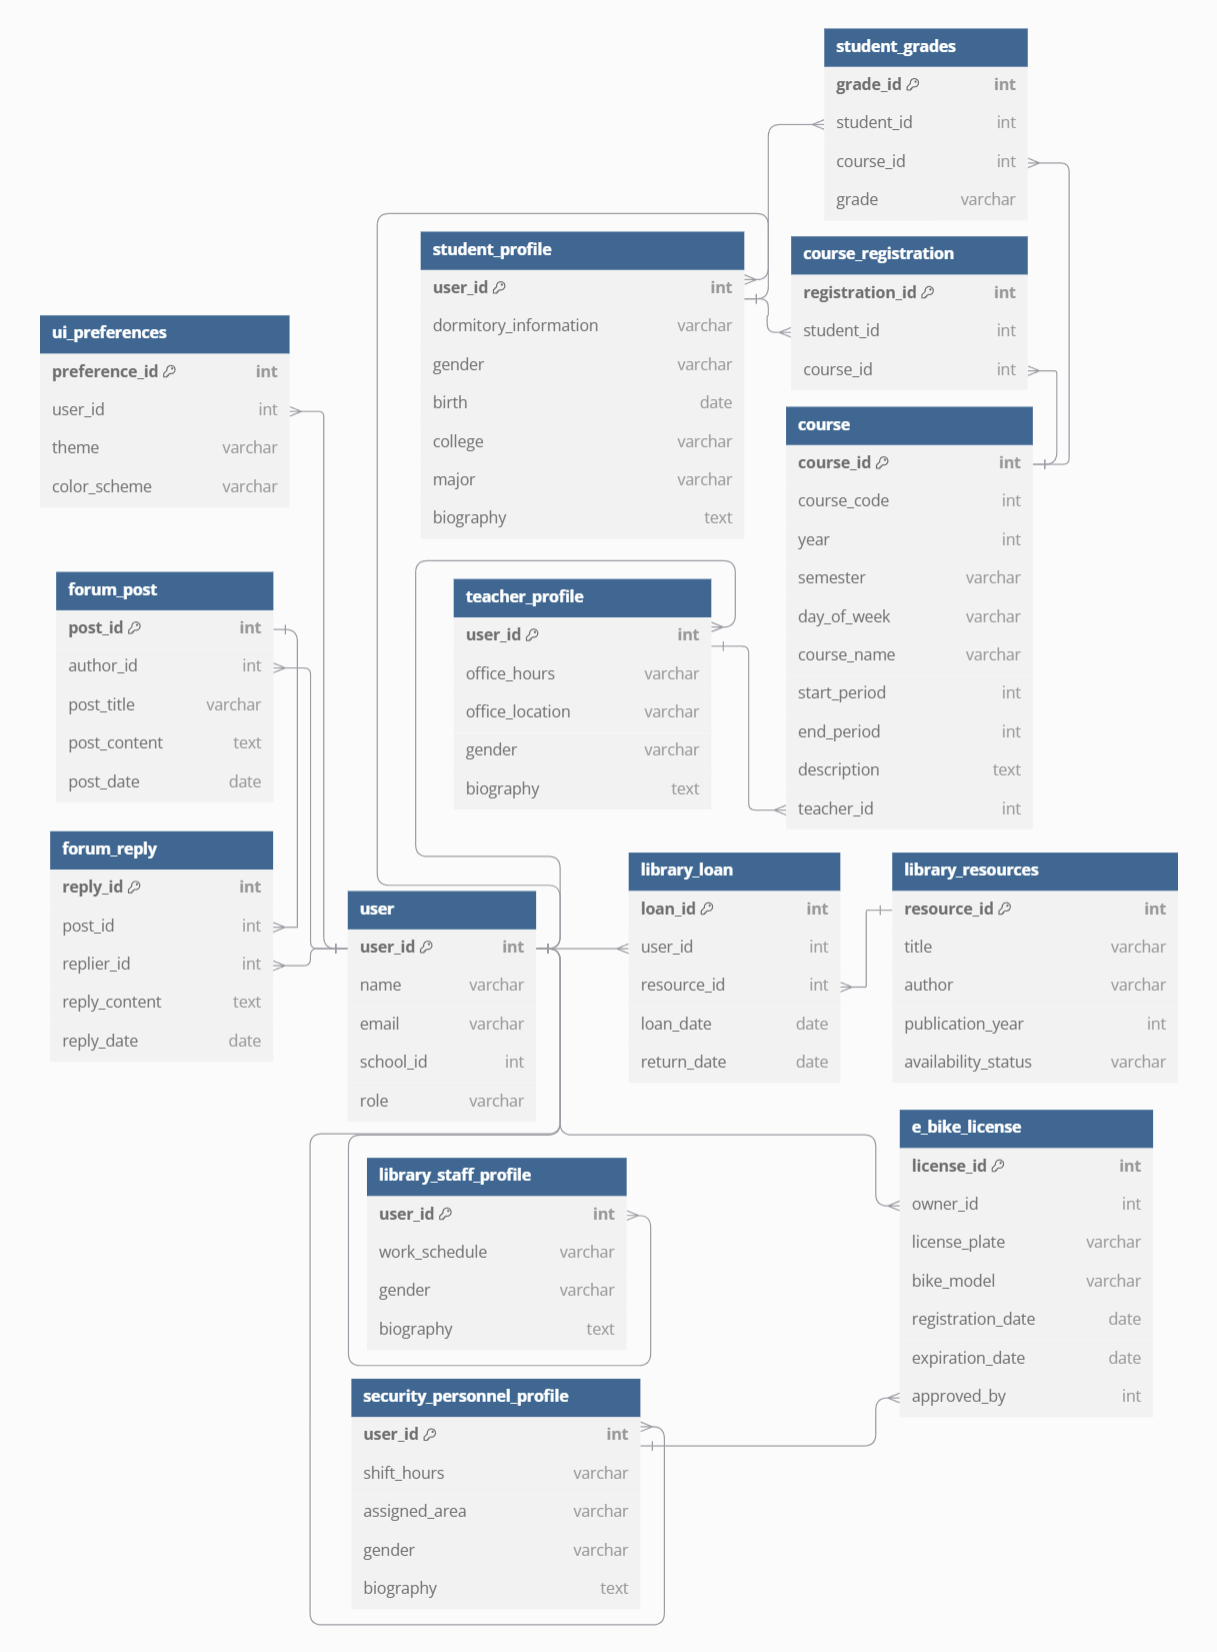
\includegraphics[width=\textwidth, height=0.8\textheight, keepaspectratio]{ER.png}
  \caption{Entity-Relationship Diagram}
\end{figure}

\clearpage  % 强制换页,并将后续内容移到图片的下一页

\subsection{Table Structures and Relationships}
Below are the current and proposed tables, along with their respective fields and relationships:

\begin{itemize}
    \item \texttt{user}: Contains user information common to all user types. Fields include:
    \begin{itemize}
        \item \texttt{user\_id} (Primary Key)
        \item \texttt{name}
        \item \texttt{email}
        \item \texttt{school\_id}
        \item \texttt{role} (e.g., student, teacher, library staff, security personnel)
    \end{itemize}
    
    \item \texttt{student\_profile}: Stores additional information specific to students. Fields include:
    \begin{itemize}
        \item \texttt{user\_id} (Foreign Key referencing \texttt{user})
        \item \texttt{dormitory\_information}
        \item \texttt{gender}
        \item \texttt{birth}
        \item \texttt{college}
        \item \texttt{major}
        \item \texttt{biography}
    \end{itemize}
    
    \item \texttt{teacher\_profile}: Stores additional information specific to teachers. Fields include:
    \begin{itemize}
        \item \texttt{user\_id} (Foreign Key referencing \texttt{user})
        \item \texttt{office\_hours}
        \item \texttt{office\_location}
        \item \texttt{gender}
        \item \texttt{biography}
    \end{itemize}
    
    \item \texttt{library\_staff\_profile}: Stores additional information specific to library staff. Fields include:
    \begin{itemize}
        \item \texttt{user\_id} (Foreign Key referencing \texttt{user})
        \item \texttt{work\_schedule}
        \item \texttt{gender}
        \item \texttt{biography}
    \end{itemize}

    \clearpage  % 强制换页,并将后续内容移到图片的下一页

    \item \texttt{security\_personnel\_profile}: Stores additional information specific to security personnel. Fields include:
    \begin{itemize}
        \item \texttt{user\_id} (Foreign Key referencing \texttt{user})
        \item \texttt{shift\_hours}
        \item \texttt{assigned\_area}
        \item \texttt{gender}
        \item \texttt{biography}
    \end{itemize}
    

    \item \texttt{course}: Contains information about the courses offered. Fields include:
    \begin{itemize}
        \item \texttt{course\_id} (Primary Key)
        \item \texttt{course\_code}
        \item \texttt{year}
        \item \texttt{semester}
        \item \texttt{day\_of\_week}
        \item \texttt{course\_name}
        \item \texttt{start\_period}
        \item \texttt{end\_period}
        \item \texttt{description}
        \item \texttt{teacher\_id} (Foreign Key referencing \texttt{teacher\_profile})
    \end{itemize}
    
    \item \texttt{course\_registration}: Tracks student registrations for courses. Fields include:
    \begin{itemize}
        \item \texttt{registration\_id} (Primary Key)
        \item \texttt{student\_id} (Foreign Key referencing \texttt{student\_profile})
        \item \texttt{course\_id} (Foreign Key referencing \texttt{course})
    \end{itemize}

    \item \texttt{student\_grades}: Stores student's grade for each course. Fields include:
    \begin{itemize}
        \item \texttt{grade\_id} (Primary Key)
        \item \texttt{student\_id} (Foreign Key referencing \texttt{student\_profile})
        \item \texttt{course\_id} (Foreign Key referencing \texttt{course})
        \item \texttt{grade} (The grade received by the student)
    \end{itemize}

    % 新增的表格
    \item \texttt{library\_resources}: Manages library books and resources. Fields include:
    \begin{itemize}
        \item \texttt{resource\_id} (Primary Key)
        \item \texttt{title}
        \item \texttt{author}
        \item \texttt{publication\_year}
        \item \texttt{availability\_status}
    \end{itemize}
    
    \item \texttt{library\_loan}: Tracks book loans by students and other users. Fields include:
    \begin{itemize}
        \item \texttt{loan\_id} (Primary Key)
        \item \texttt{user\_id} (Foreign Key referencing \texttt{user})
        \item \texttt{resource\_id} (Foreign Key referencing \texttt{library\_resources})
        \item \texttt{loan\_date}
        \item \texttt{return\_date}
    \end{itemize}
    
    \item \texttt{e\_bike\_license}: Manages electric bike licenses for students, teachers, and library staff. Fields include:
    \begin{itemize}
        \item \texttt{license\_id} (Primary Key)
        \item \texttt{owner\_id} (Foreign Key referencing \texttt{user})
        \item \texttt{license\_plate}
        \item \texttt{bike\_model}
        \item \texttt{registration\_date}
        \item \texttt{expiration\_date}
        \item \texttt{approved\_by} (Foreign Key referencing \texttt{security\_personnel\_profile})
    \end{itemize}

    \item \texttt{forum\_post}: Stores user-created posts for the forum. Fields include:
    \begin{itemize}
        \item \texttt{post\_id} (Primary Key)
        \item \texttt{author\_id} (Foreign Key referencing \texttt{user})
        \item \texttt{post\_title}
        \item \texttt{post\_content}
        \item \texttt{post\_date}
    \end{itemize}
    
    \item \texttt{forum\_reply}: Stores user replies to forum posts. Fields include:
    \begin{itemize}
        \item \texttt{reply\_id} (Primary Key)
        \item \texttt{post\_id} (Foreign Key referencing \texttt{forum\_post})
        \item \texttt{replier\_id} (Foreign Key referencing \texttt{user})
        \item \texttt{reply\_content}
        \item \texttt{reply\_date}
    \end{itemize}

    \item \texttt{ui\_preferences}: Stores user preferences for the UI interface. Fields include:
    \begin{itemize}
        \item \texttt{preference\_id} (Primary Key)
        \item \texttt{user\_id} (Foreign Key referencing \texttt{user})
        \item \texttt{theme} (Preferred UI theme, e.g., light, dark)
        \item \texttt{color\_scheme} (Preferred color scheme, e.g., blue, green)
    \end{itemize}
\end{itemize}

\subsection{Primary and Foreign Key Design}
Each table contains a primary key that uniquely identifies each record. Foreign keys are used to establish relationships between users and the entities they interact with. For example:
\begin{itemize}
    \item The \texttt{user\_id} field in \texttt{student\_profile}, \texttt{teacher\_profile}, 
    \texttt{library\_staff\_profile}, and \texttt{security\_personnel\_profile} links the 
    profiles to the core \texttt{user} table.
    \item The \texttt{course\_id} field in \texttt{course\_registration} and \texttt{student\_grades} links 
    students to the courses they have enrolled in and the grades they have received.
    \item The \texttt{license\_id} in the \texttt{e\_bike\_license} table allows students 
    to register electric bikes, which are approved by security personnel.
    \item The \texttt{post\_id} and \texttt{reply\_id} in the \texttt{forum\_post} and \texttt{forum\_reply} 
    tables link forum posts and their replies to the users who created them.
    \item The \texttt{user\_id} field in the \texttt{ui\_preferences} table links users to their personalized 
    interface settings, such as theme, font size, and color scheme.
\end{itemize}

\subsection{Data Population Strategy}
The initial data for the \texttt{user}, \texttt{course}, and \texttt{library\_resources} 
tables will be seeded by administrators during development and testing phases. As users 
interact with the system, data will be dynamically added to the \texttt{course\_registration}, 
\texttt{student\_grades}, \texttt{library\_loan}, \texttt{e\_bike\_license}, \texttt{forum\_post}, 
\texttt{forum\_reply}, and \texttt{ui\_preferences} tables. The system will ensure that all data 
remains up-to-date and consistent across these entities, allowing users to track their course 
registrations, grades, library loans, and personalized interface preferences.

\newpage
\section{Web Page Design}
\subsection{Overview}

The following sections provide an overview of the user interface elements. The \textit{Mockups for common functions} subsection presents interfaces accessible by multiple user types, such as the library search page and profile management. Subsequent sections detail user-specific interfaces, including course management for teachers and e-bike registration for students.

\subsection{Mockups for common functions}

\begin{figure}[H]
    \centering
    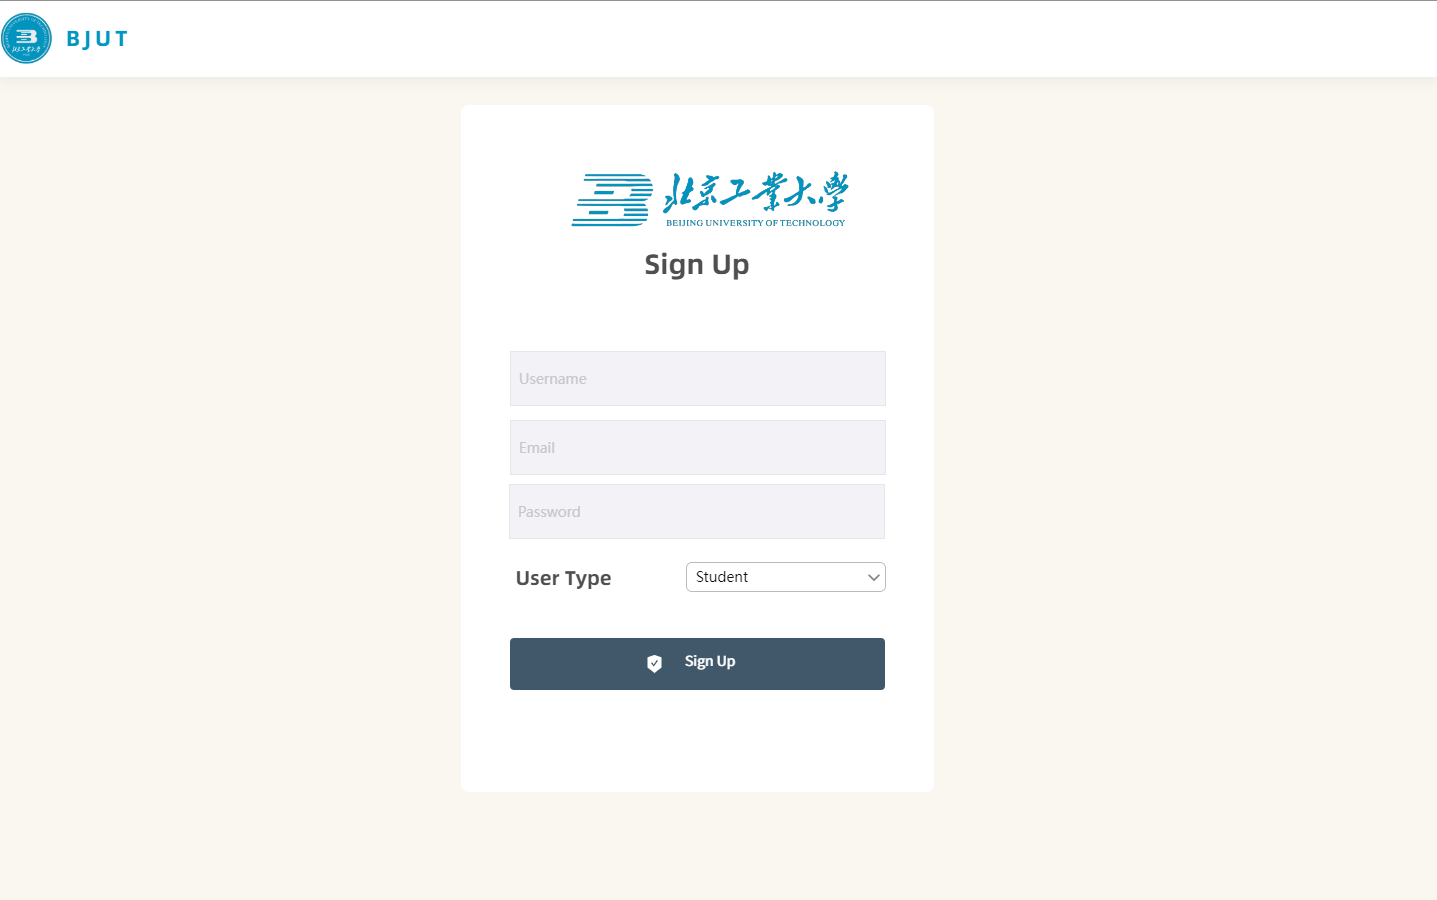
\includegraphics[width=\textwidth]{mockups/common/register.png}
    \caption{Register Page}
    \label{fig:register_page}
\end{figure}

\begin{figure}[H]
    \centering
    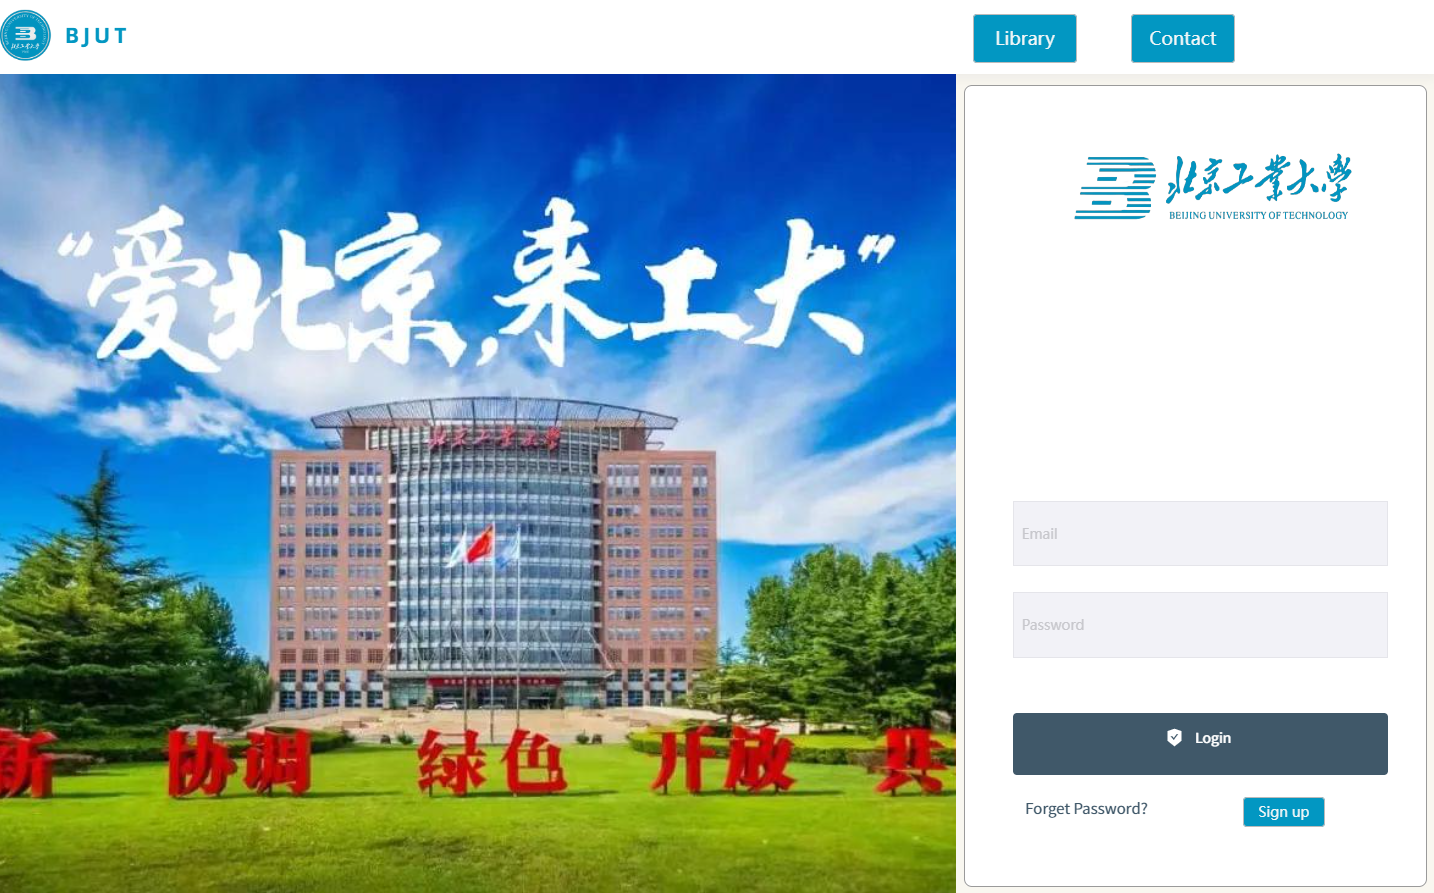
\includegraphics[width=\textwidth]{mockups/common/login.png}
    \caption{Login Page}
    \label{fig:login_page}
\end{figure}

\begin{figure}[H]
    \centering
    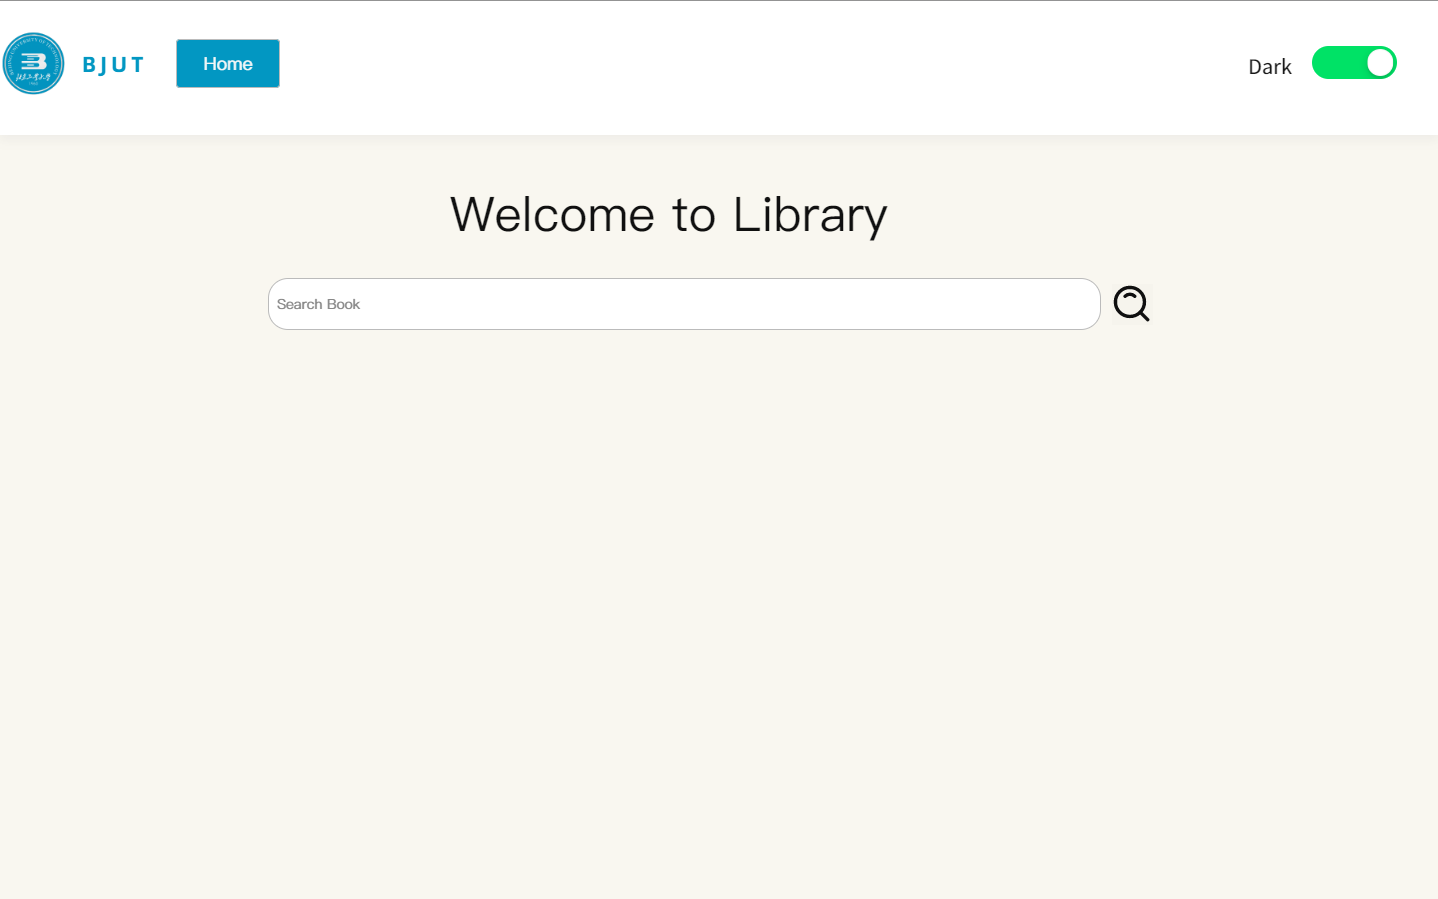
\includegraphics[width=\textwidth]{mockups/common/searchbook.png}
    \caption{Book Searching Page}
    \label{fig:searchbook_page}
\end{figure}

\begin{figure}[H]
    \centering
    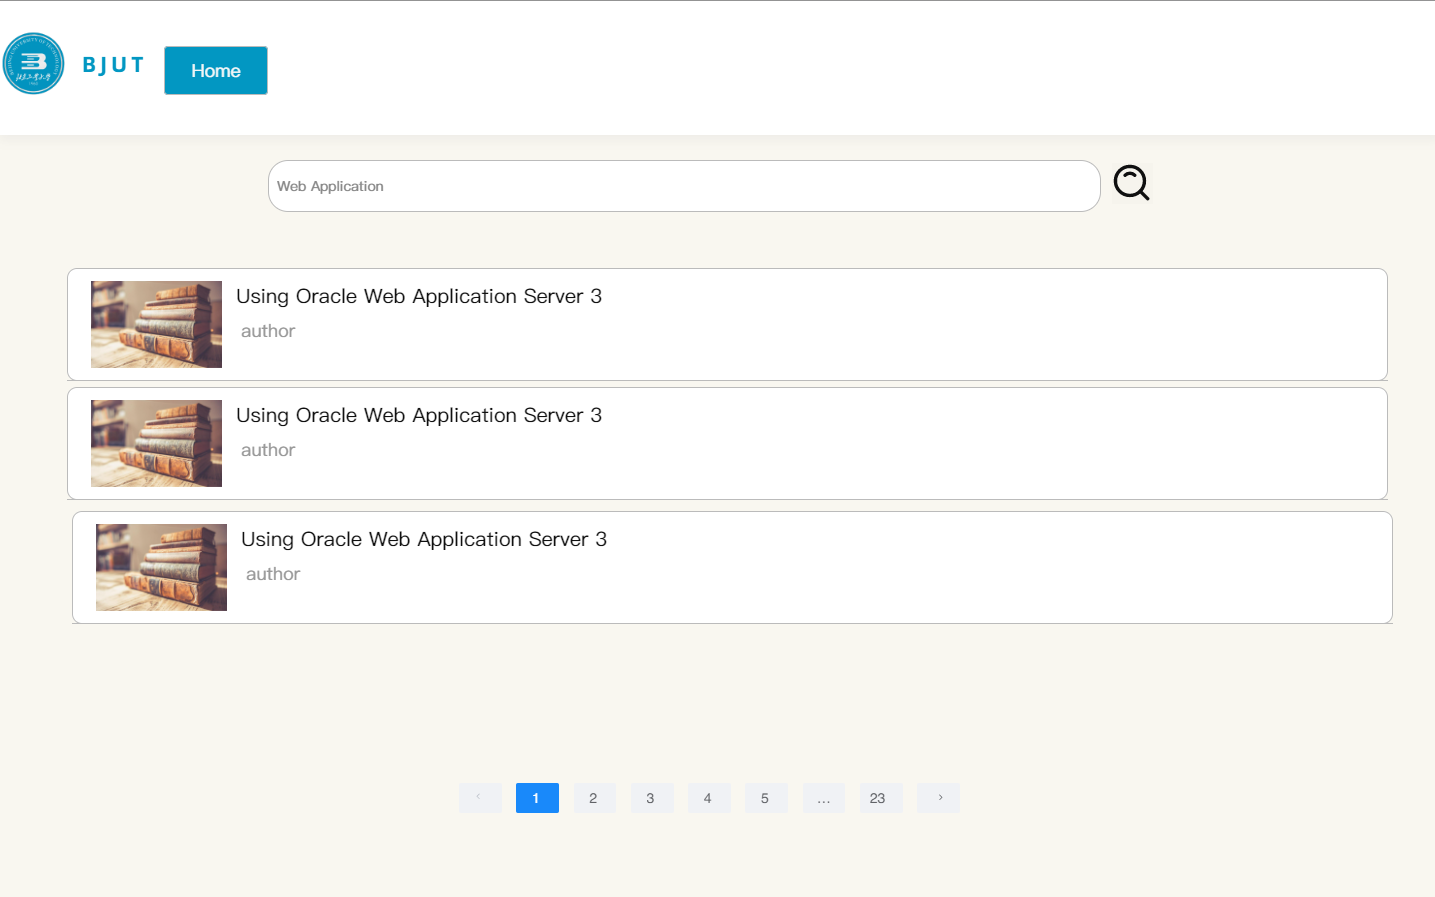
\includegraphics[width=\textwidth]{mockups/common/searchbookresult.png}
    \caption{Book Searching Result Page}
    \label{fig:searchbookresult_page}
\end{figure}

\begin{figure}[H]
    \centering
    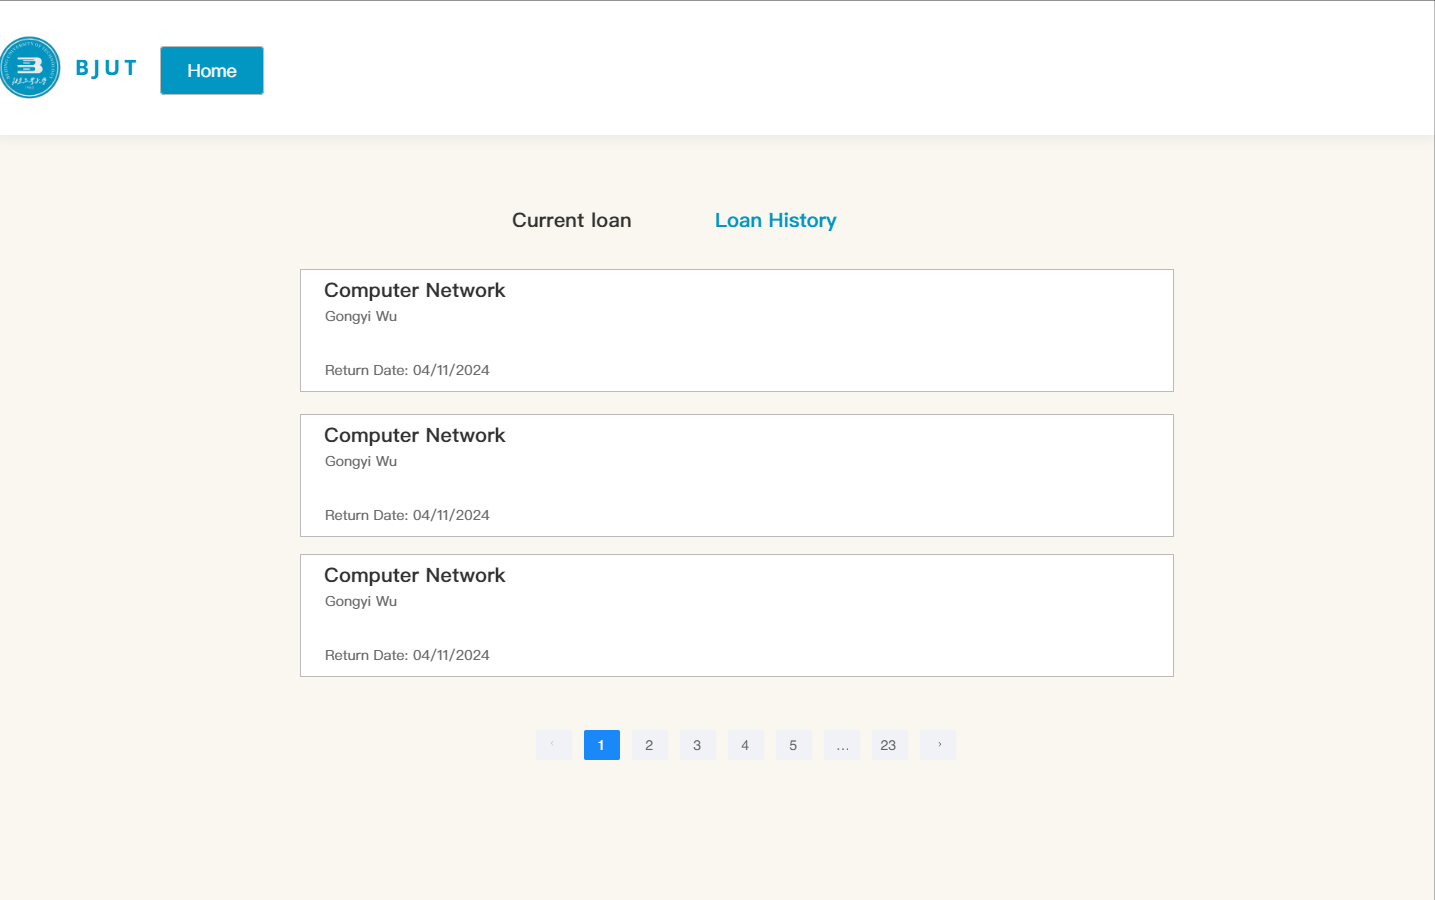
\includegraphics[width=\textwidth]{mockups/common/loanrecord.png}
    \caption{Loan Record Page}
    \label{fig:loanrecord_page}
\end{figure}

\begin{figure}[H]
    \centering
    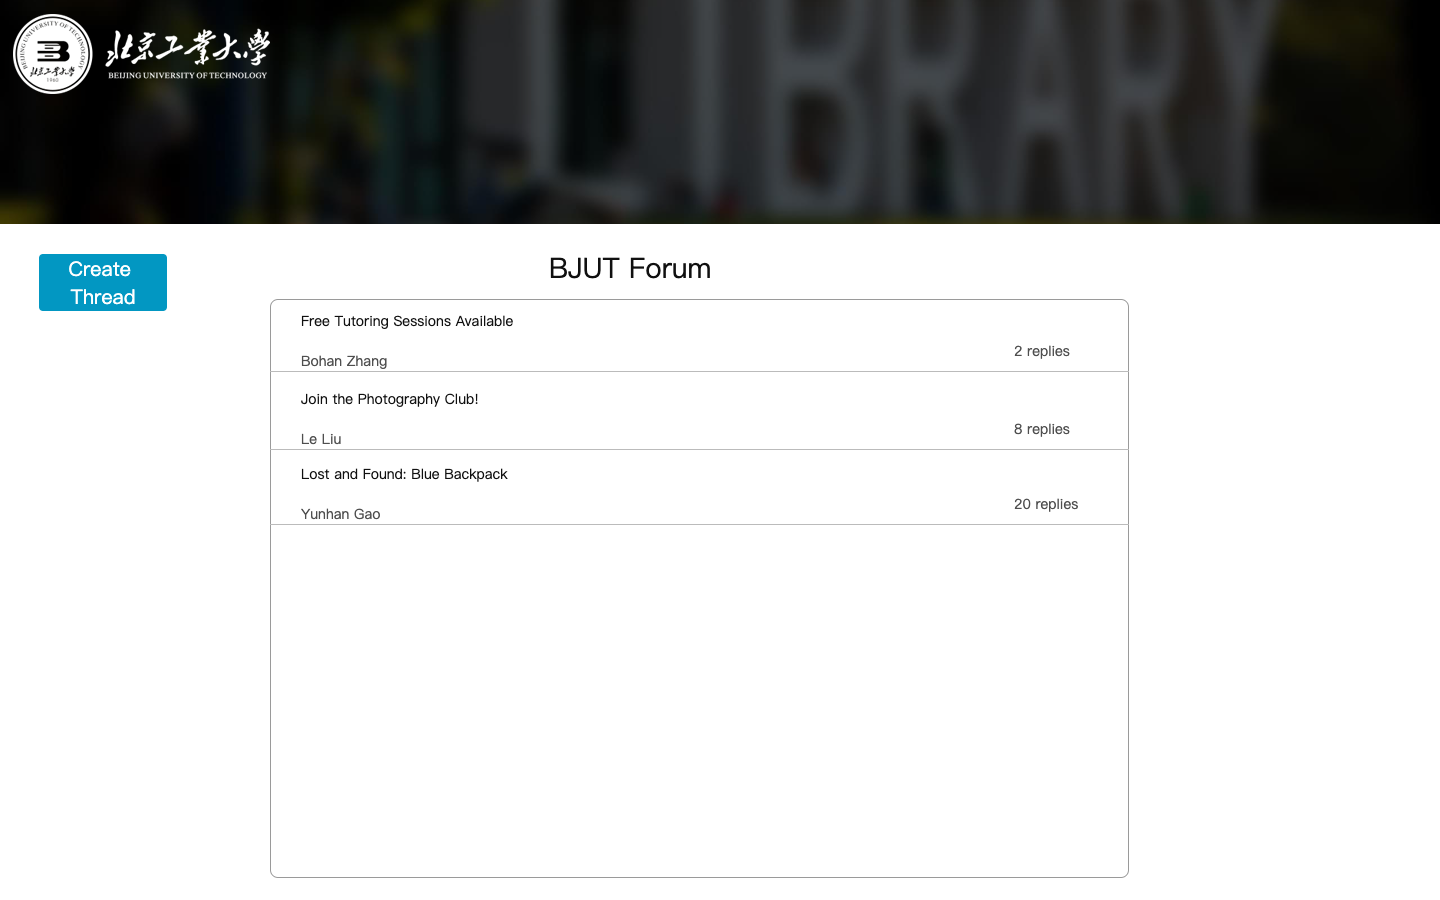
\includegraphics[width=\textwidth]{mockups/common/forum.png}
    \caption{Forum Page}
    \label{fig:forum_page}
\end{figure}

\begin{figure}[H]
    \centering
    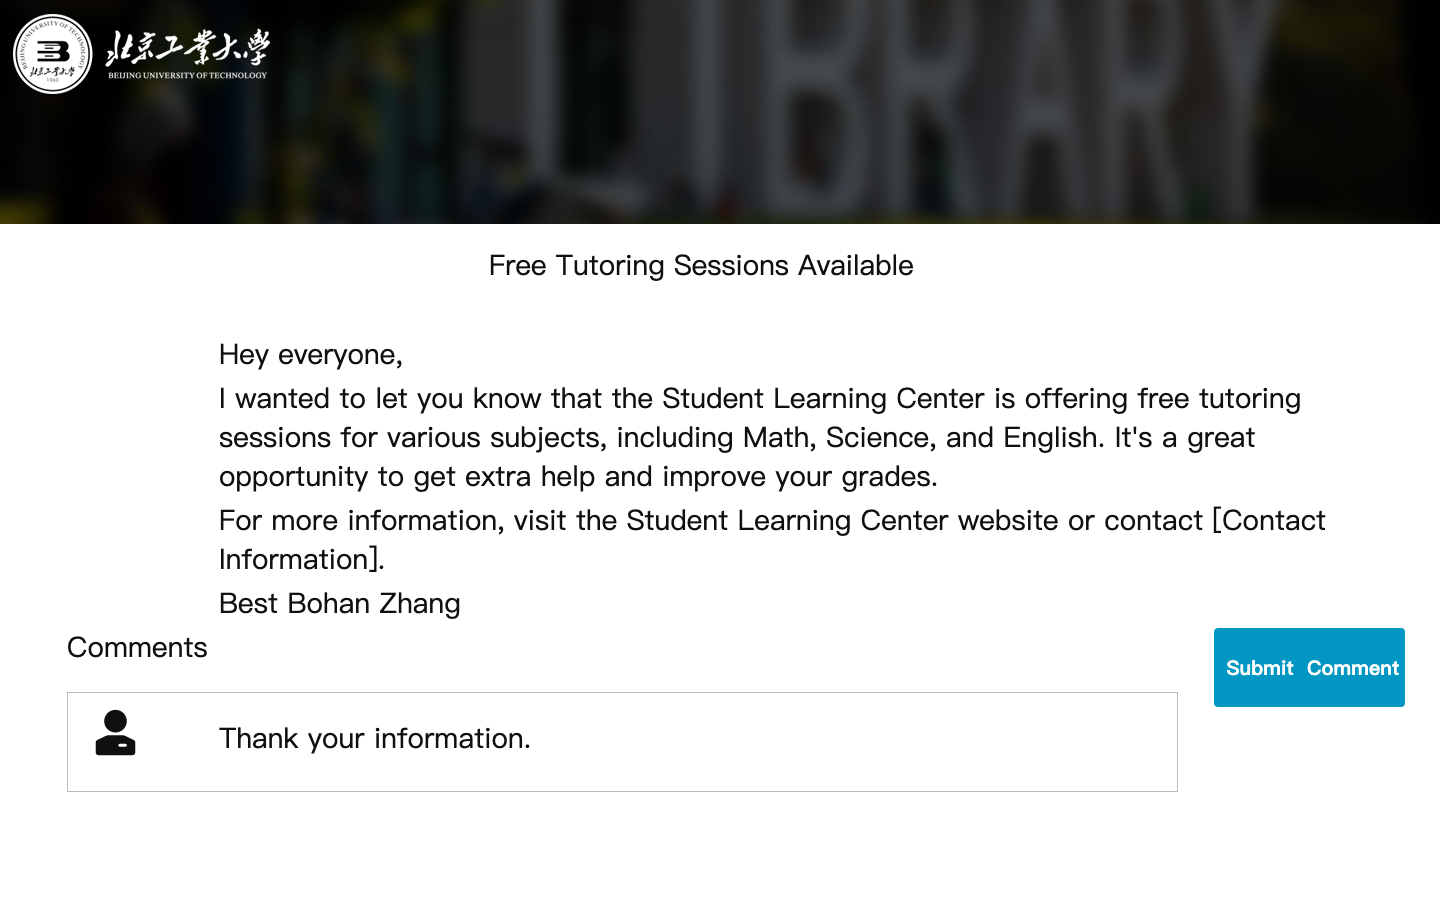
\includegraphics[width=\textwidth]{mockups/common/forumdetail.png}
    \caption{Forum Detail Page}
    \label{fig:forudetail_page}
\end{figure}

\begin{figure}[H]
    \centering
    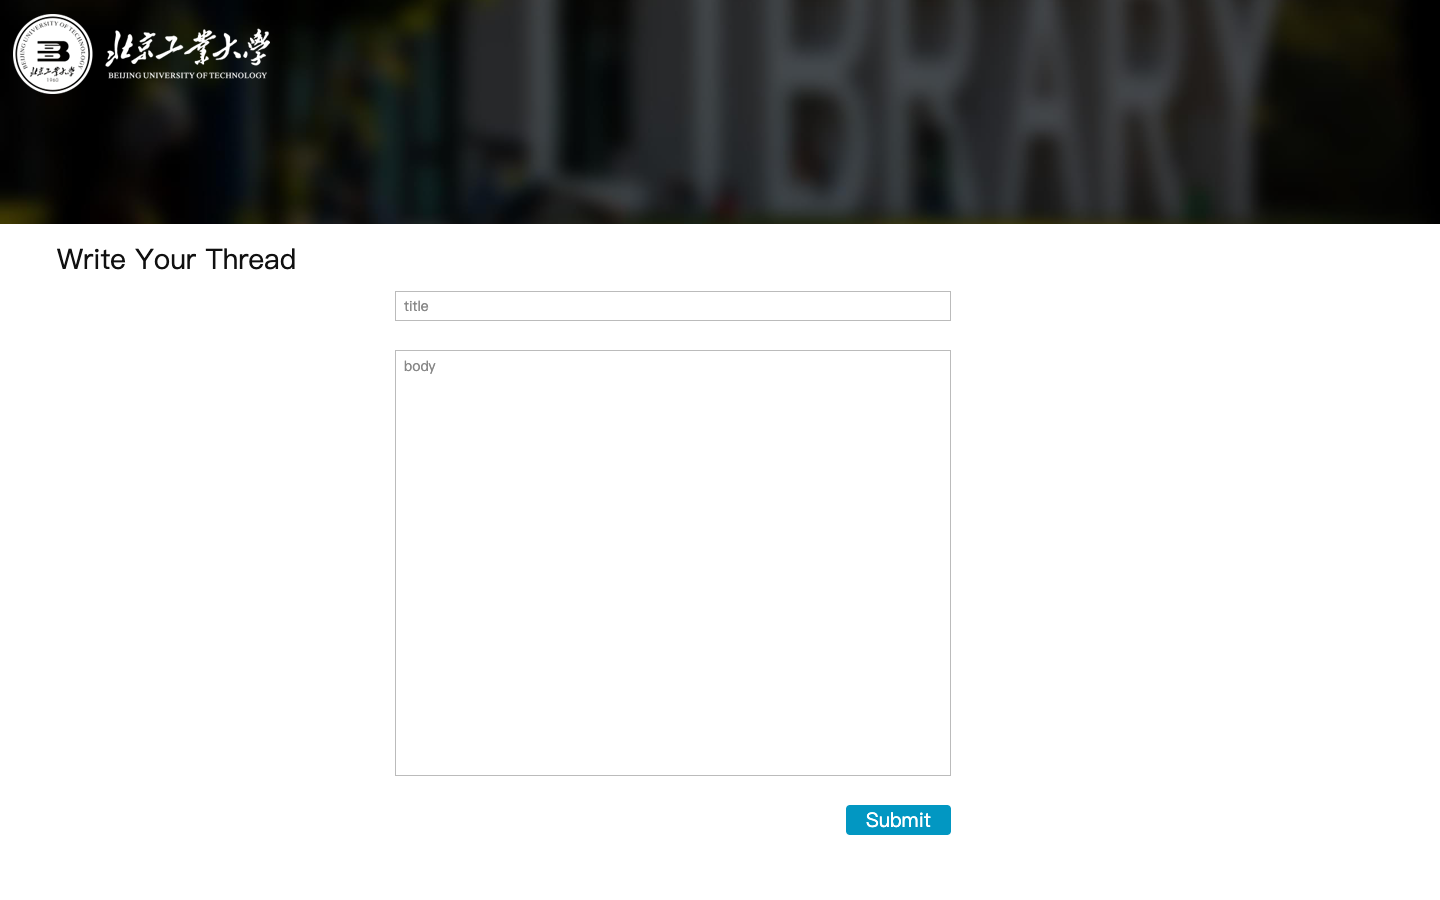
\includegraphics[width=\textwidth]{mockups/common/postforum.png}
    \caption{Posting Page}
    \label{fig:posting_page}
\end{figure}

\subsection{Mockups for student functions}

\begin{figure}[H]
    \centering
    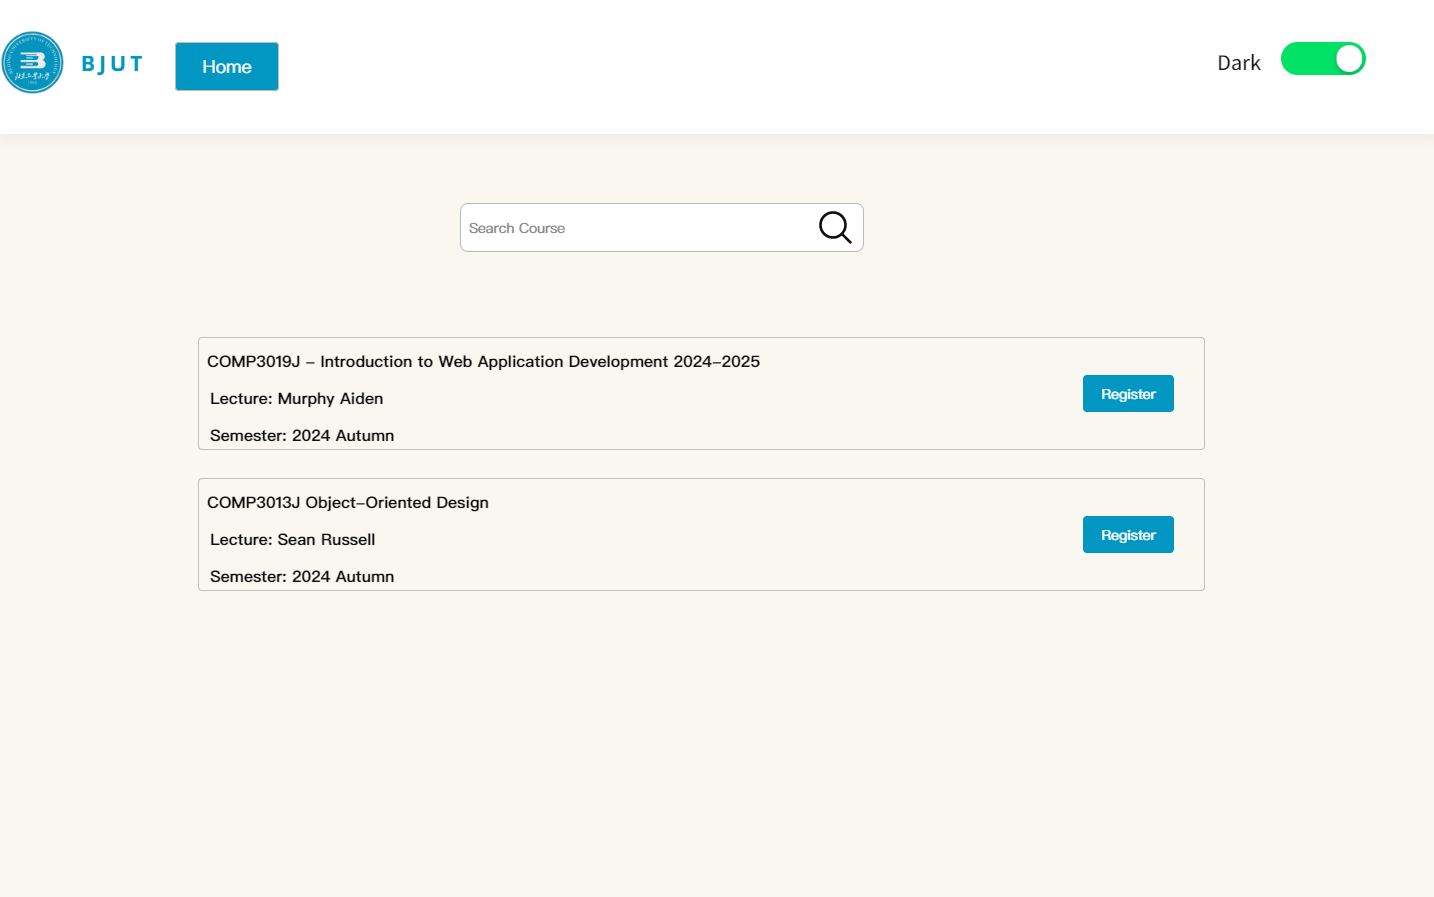
\includegraphics[width=\textwidth]{mockups/student/addcourse.png}
    \caption{Add Course Page}
    \label{fig:addcourse_page}
\end{figure}

\begin{figure}[H]
    \centering
    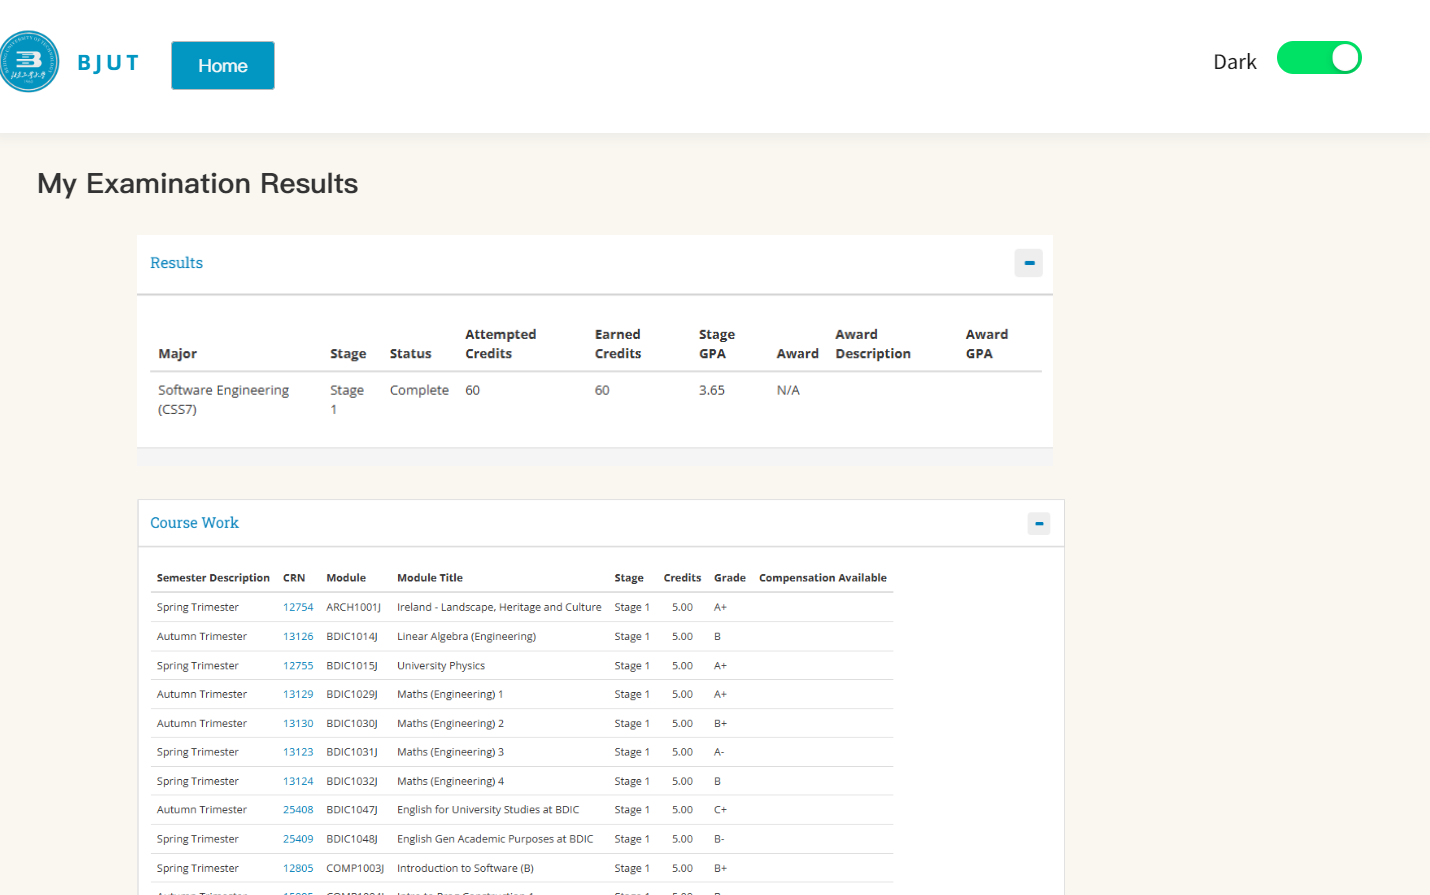
\includegraphics[width=\textwidth]{mockups/student/grade.png}
    \caption{Grade Page}
    \label{fig:grade_page}
\end{figure}

\begin{figure}[H]
    \centering
    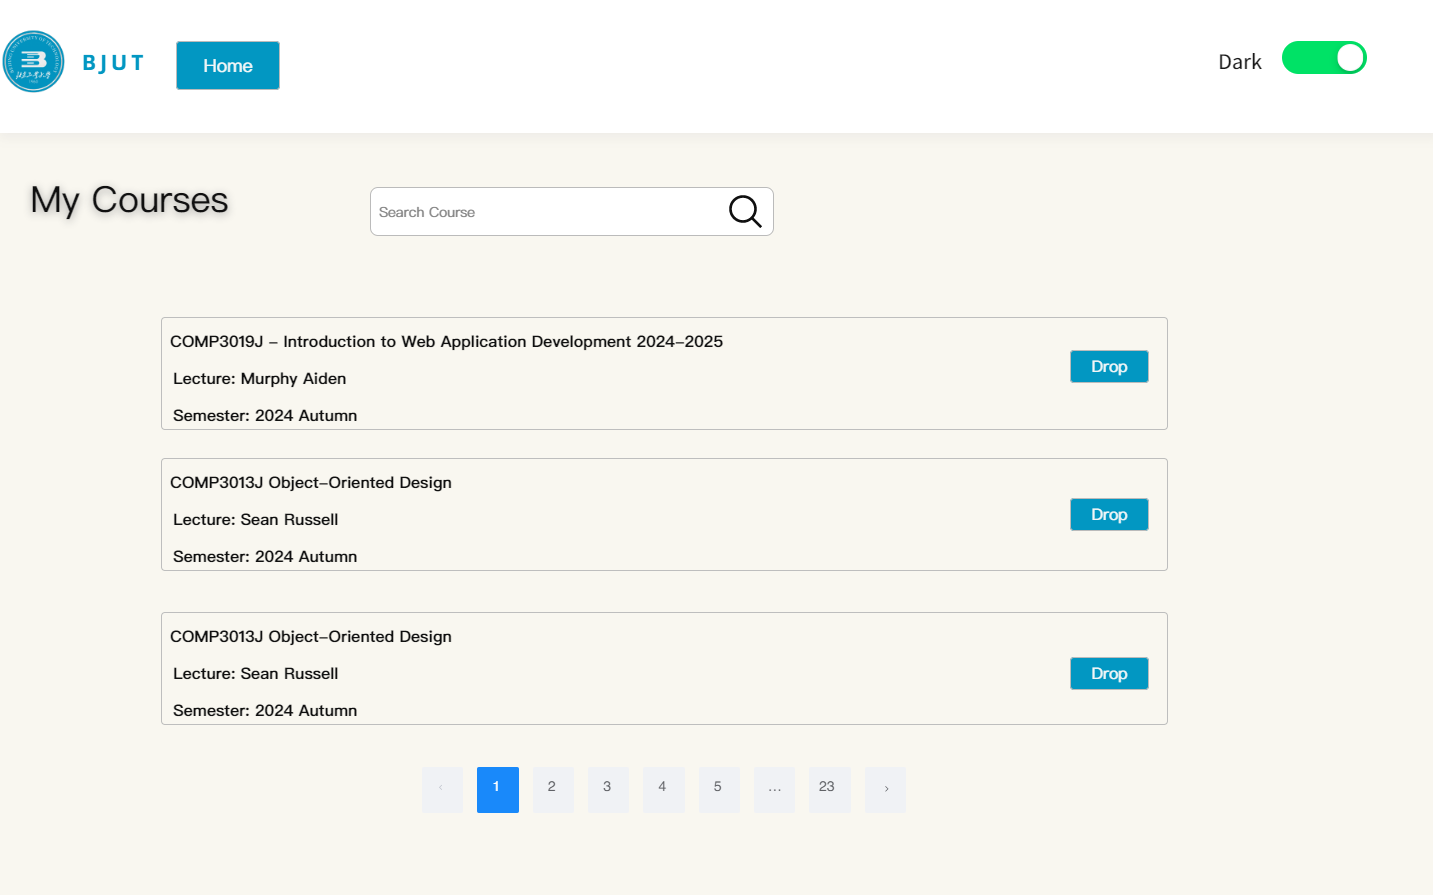
\includegraphics[width=\textwidth]{mockups/student/mycourse.png}
    \caption{My Course Page}
    \label{fig:mycourse_page}
\end{figure}

\begin{figure}[H]
    \centering
    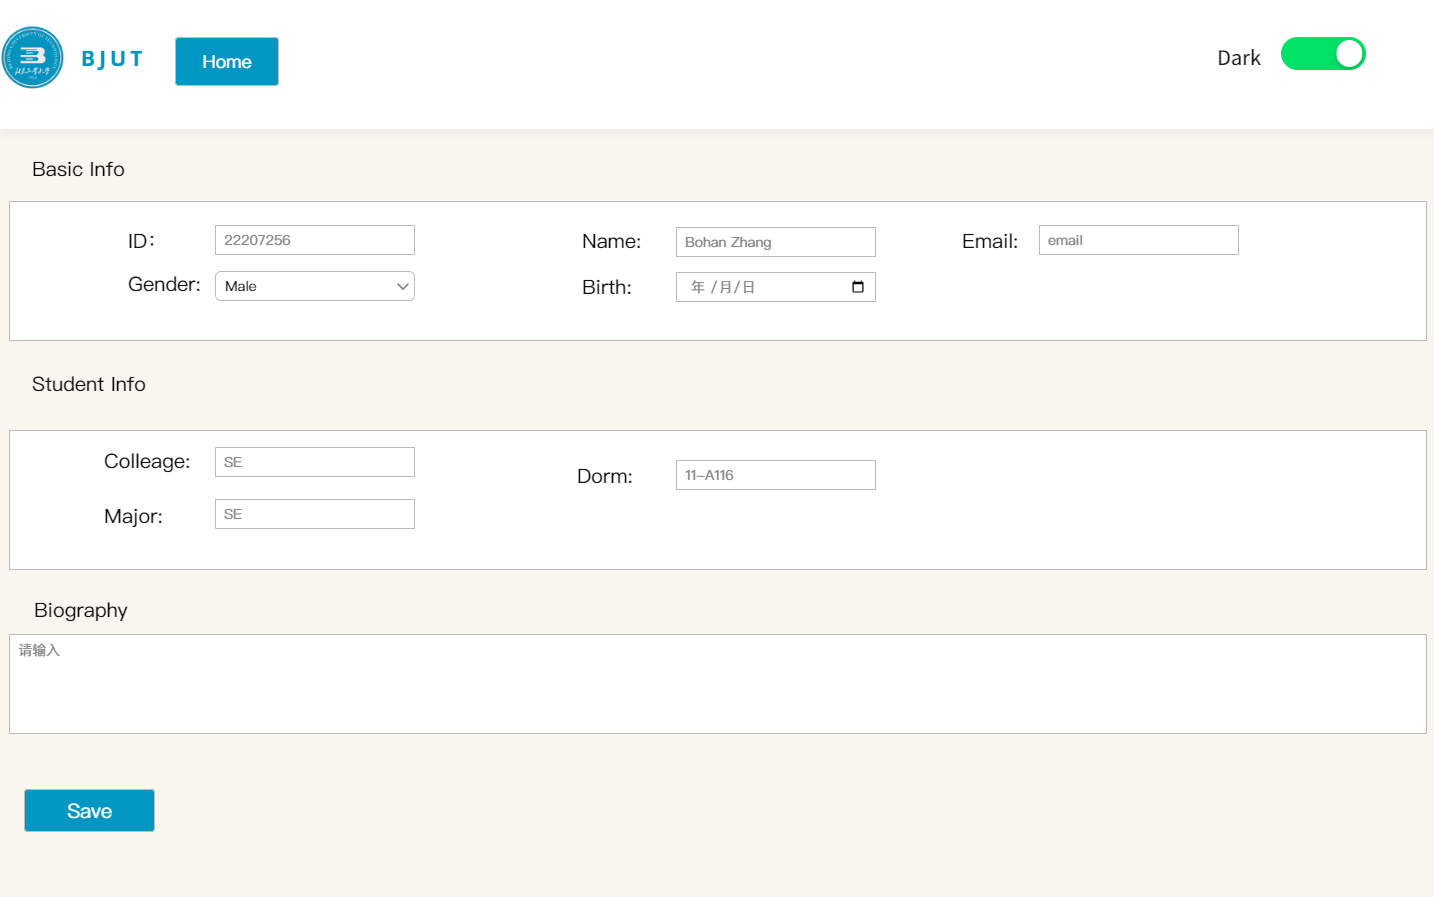
\includegraphics[width=\textwidth]{mockups/student/profile.png}
    \caption{Profile Page}
    \label{fig:student_profile_page}
\end{figure}

\begin{figure}[H]
    \centering
    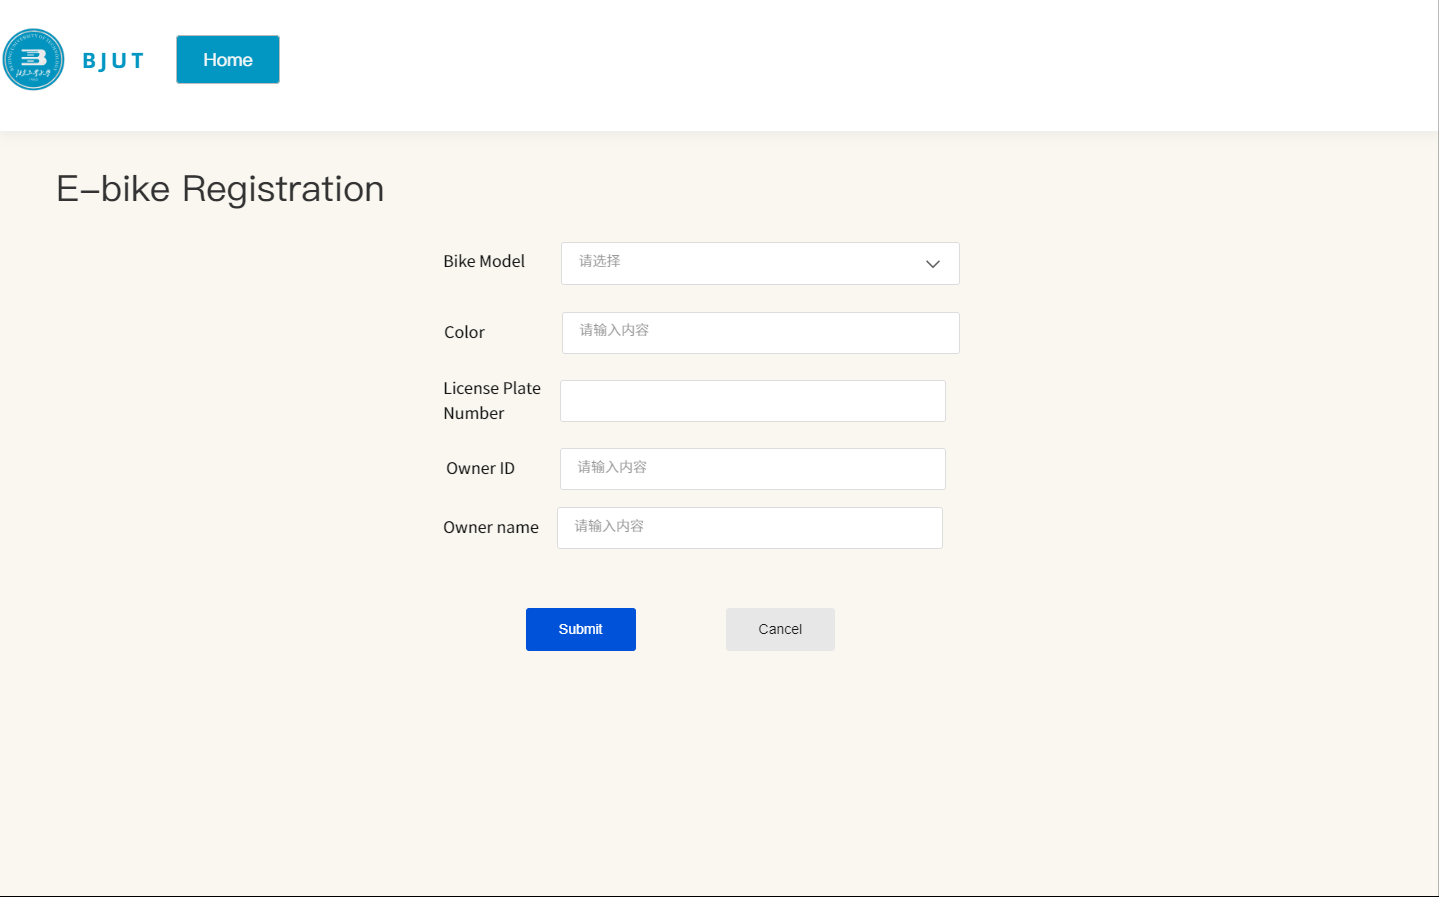
\includegraphics[width=\textwidth]{mockups/student/registerebike.png}
    \caption{E-bike Registration Page}
    \label{fig:registerebike_page}
\end{figure}

\begin{figure}[H]
    \centering
    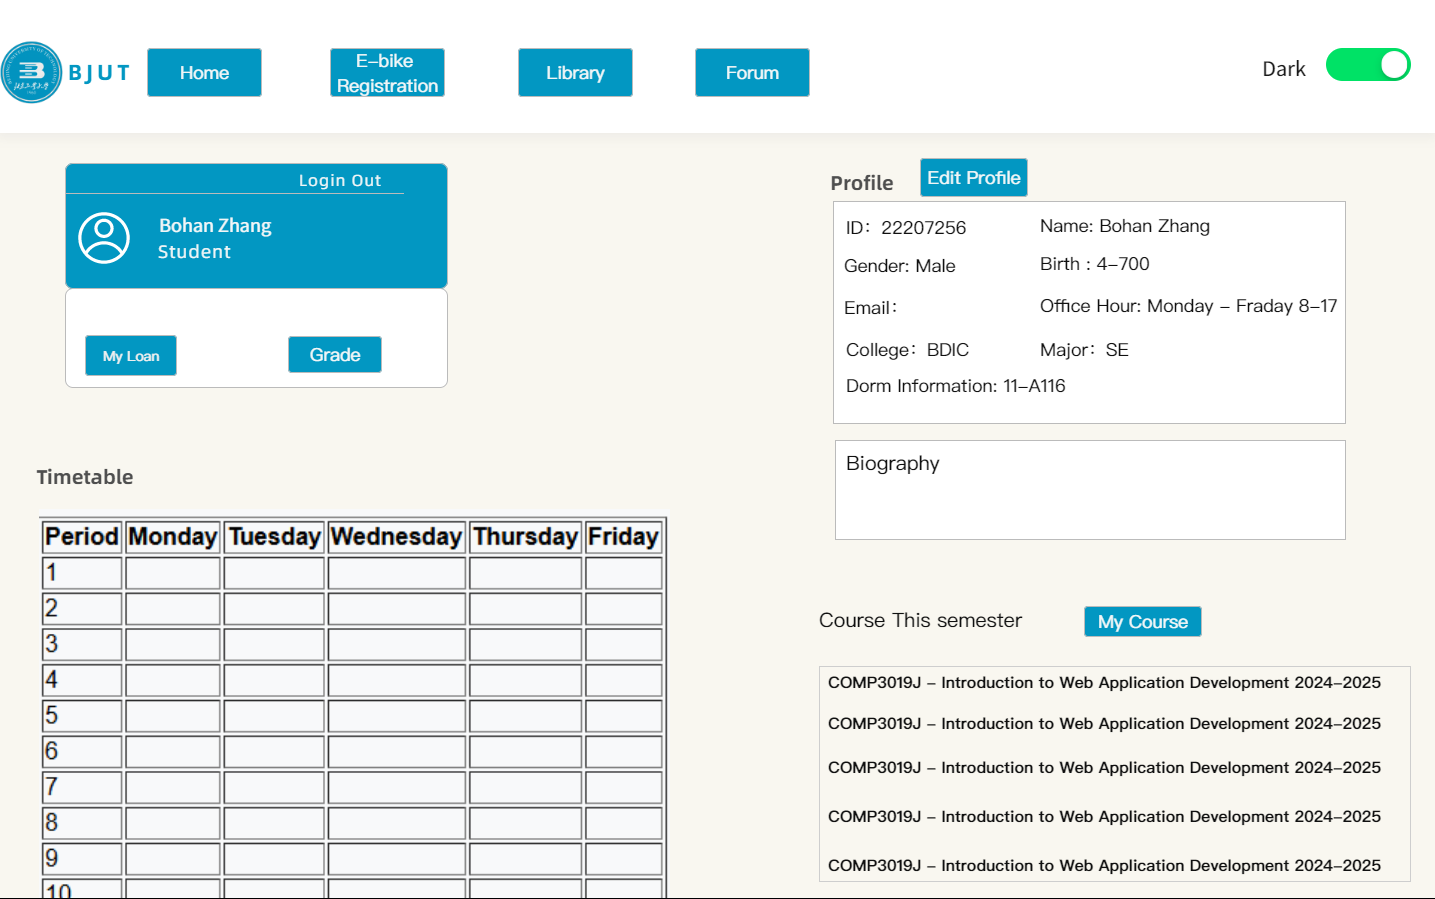
\includegraphics[width=\textwidth]{mockups/student/studentdash.png}
    \caption{Student Dashboard}
    \label{fig:student_dashboard}
\end{figure}


\subsection{Mockups for teacher functions}

\begin{figure}[H]
    \centering
    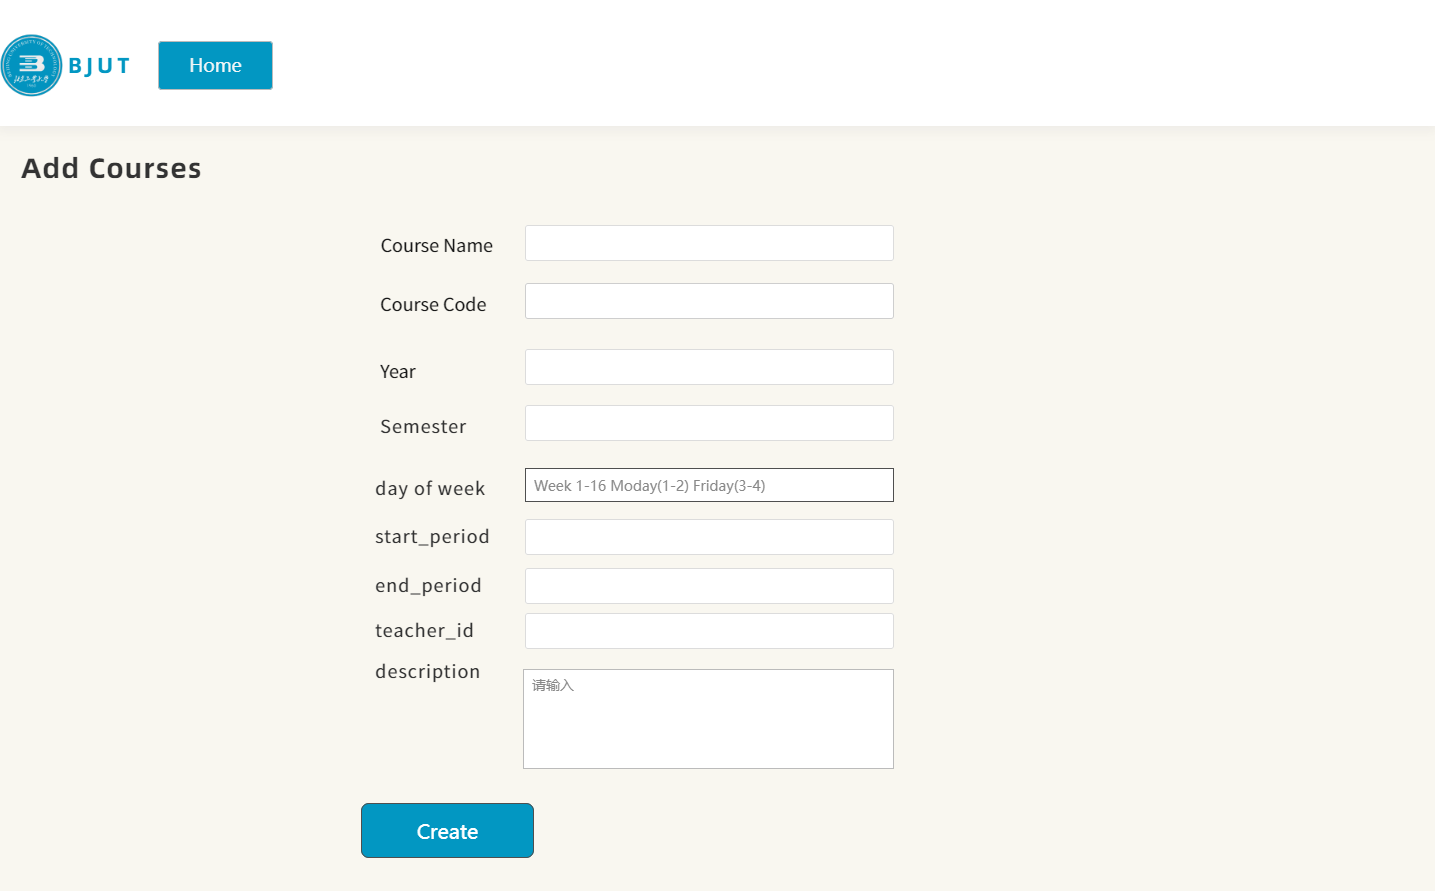
\includegraphics[width=\textwidth]{mockups/teacher/addcourse.png}
    \caption{Add Course Page (Teacher)}
    \label{fig:teacher_addcourse_page}
\end{figure}

\begin{figure}[H]
    \centering
    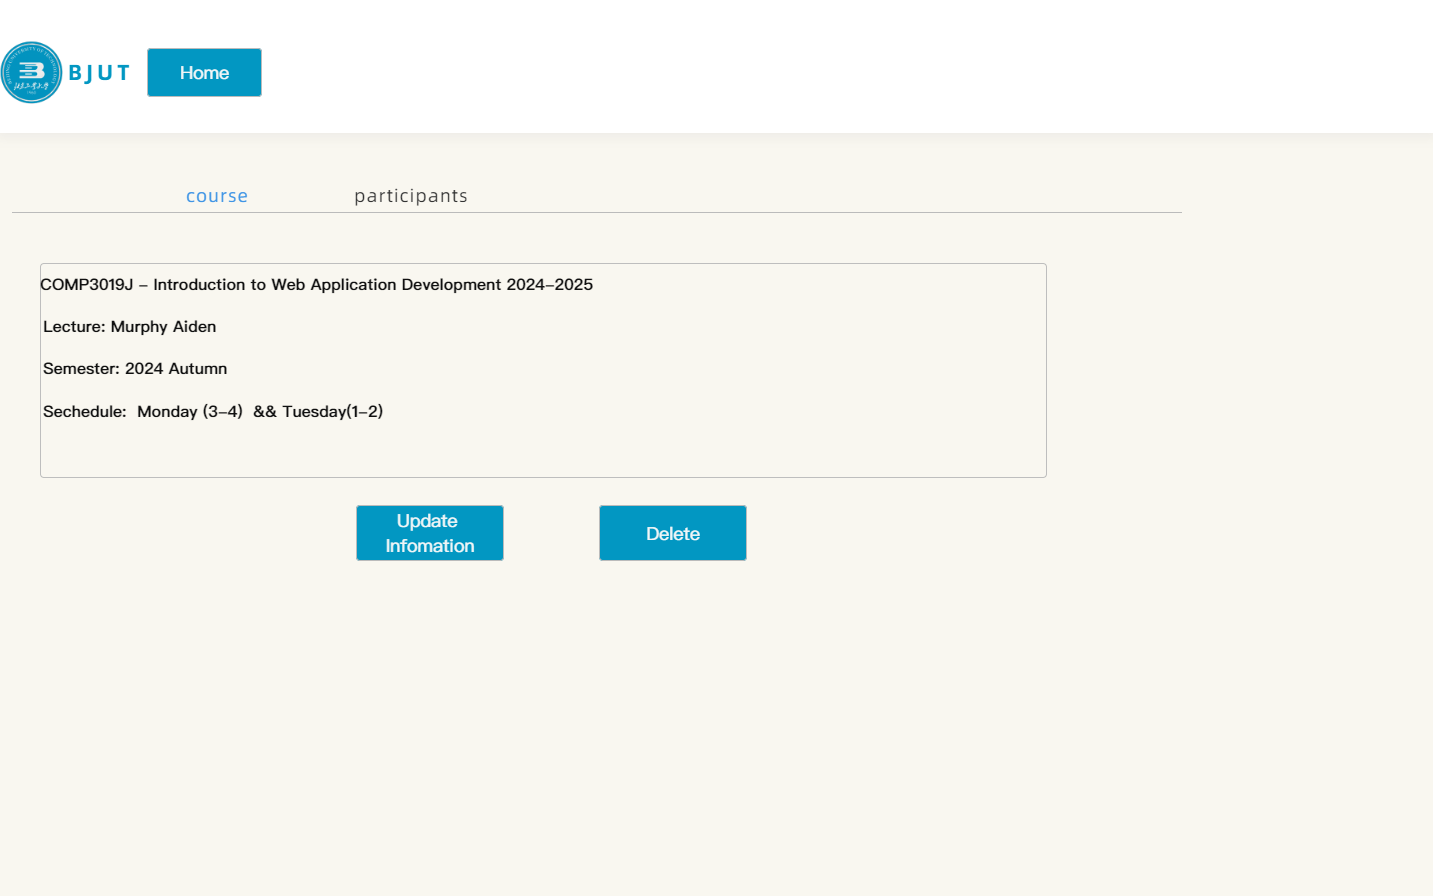
\includegraphics[width=\textwidth]{mockups/teacher/coursedetail.png}
    \caption{Course Detail Page}
    \label{fig:teacher_coursedetail_page}
\end{figure}

\begin{figure}[H]
    \centering
    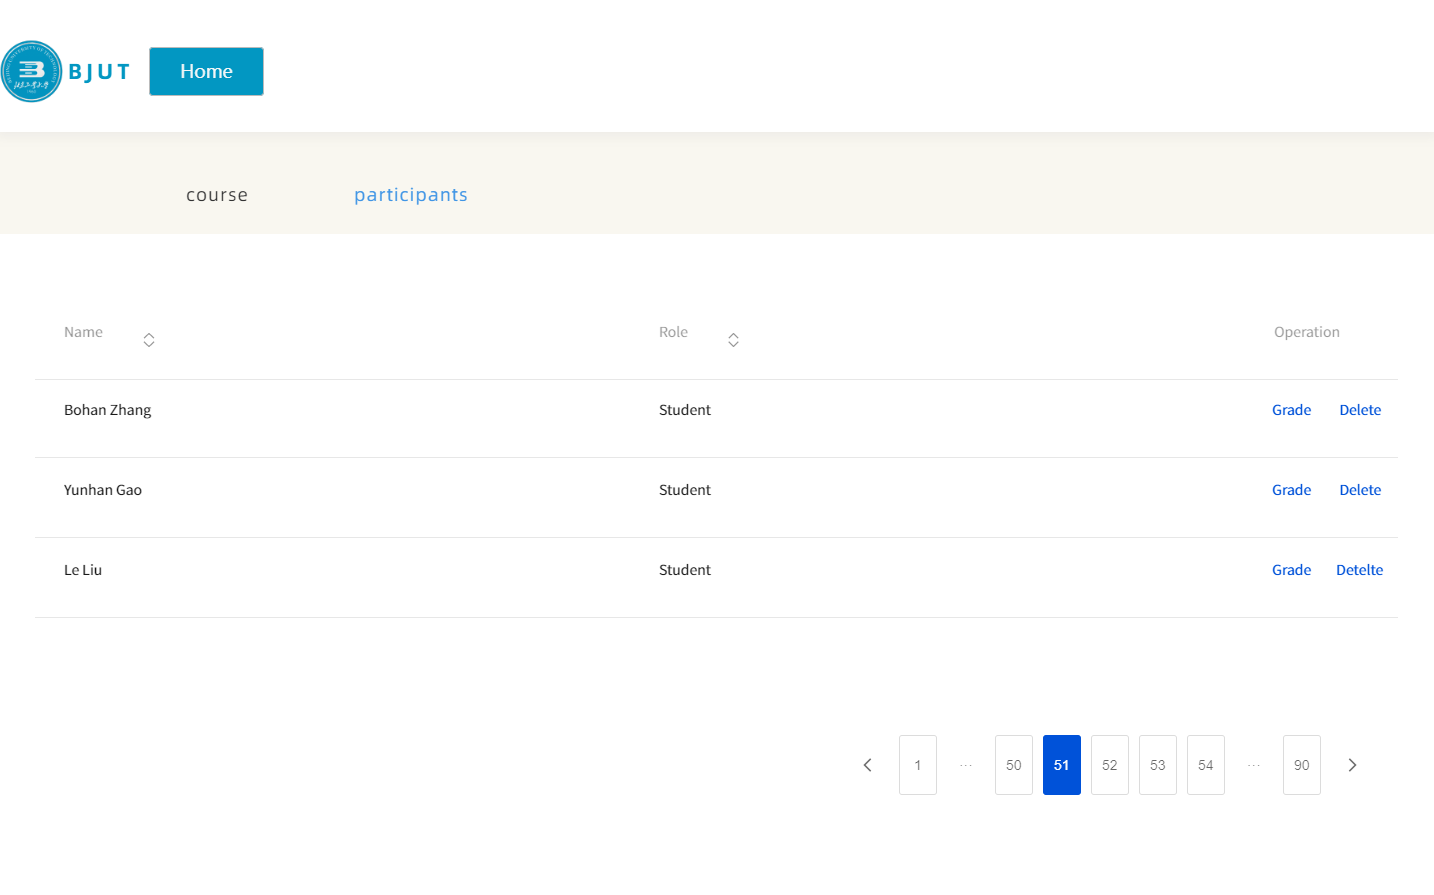
\includegraphics[width=\textwidth]{mockups/teacher/grade.png}
    \caption{Grade Page}
    \label{fig:teacher_grade_page}
\end{figure}

\begin{figure}[H]
    \centering
    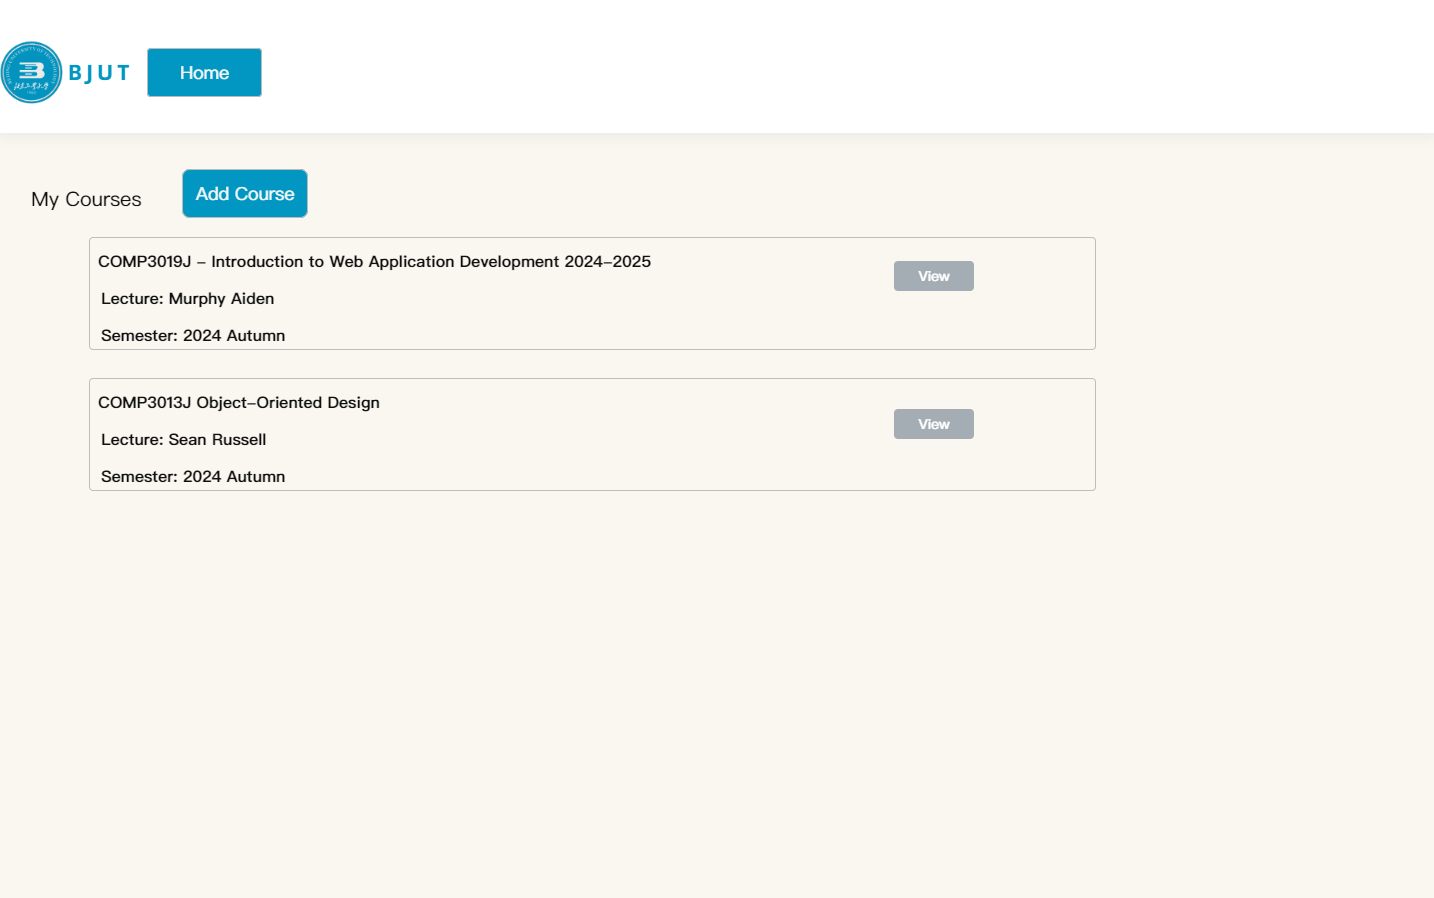
\includegraphics[width=\textwidth]{mockups/teacher/mycourses.png}
    \caption{My Courses Page}
    \label{fig:teacher_mycourses_page}
\end{figure}

\begin{figure}[H]
    \centering
    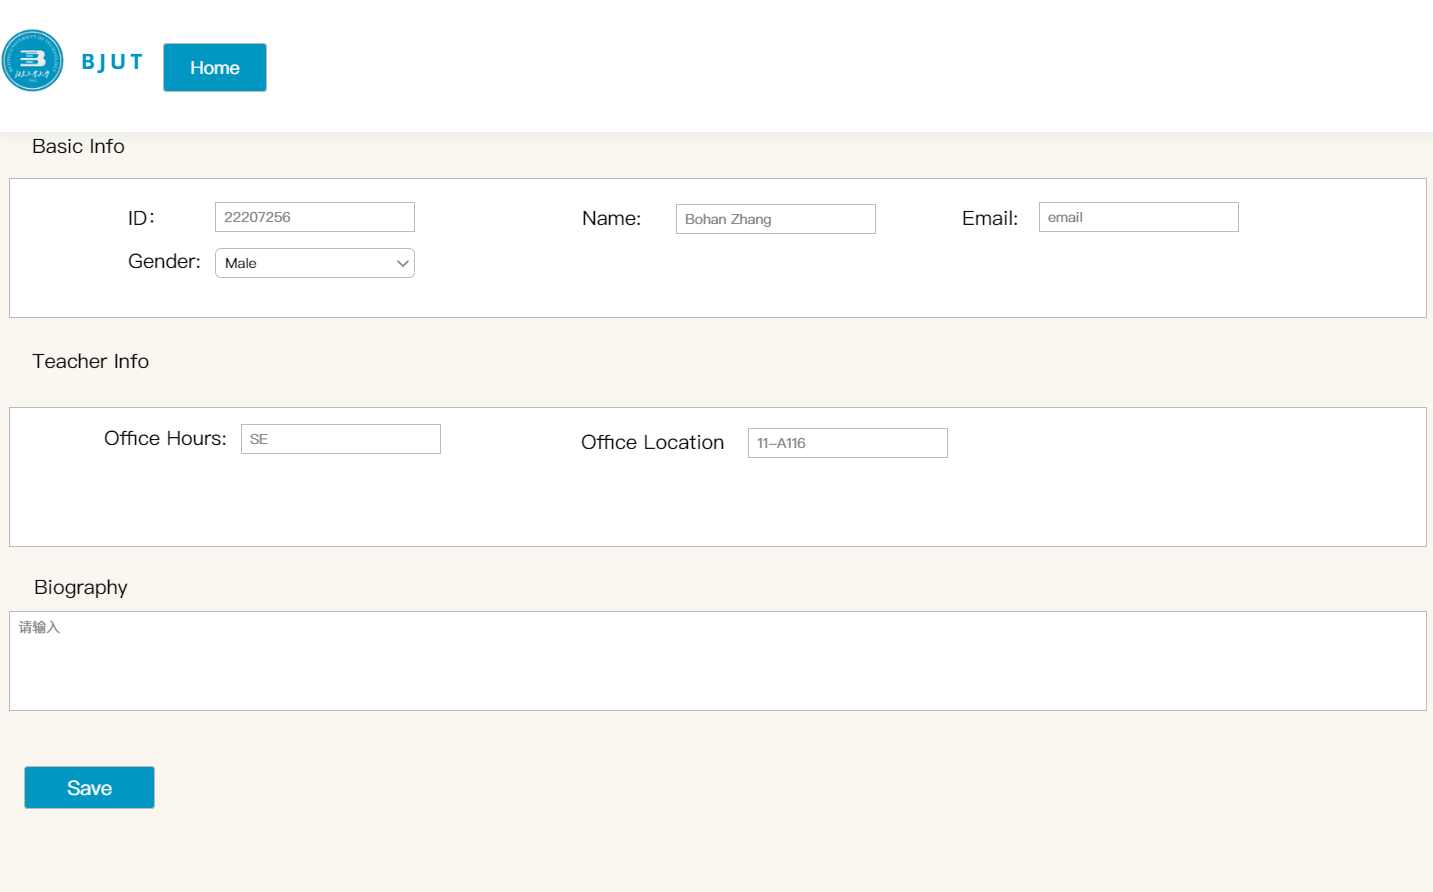
\includegraphics[width=\textwidth]{mockups/teacher/profile.png}
    \caption{Profile Page}
    \label{fig:teacher_profile_page}
\end{figure}

\begin{figure}[H]
    \centering
    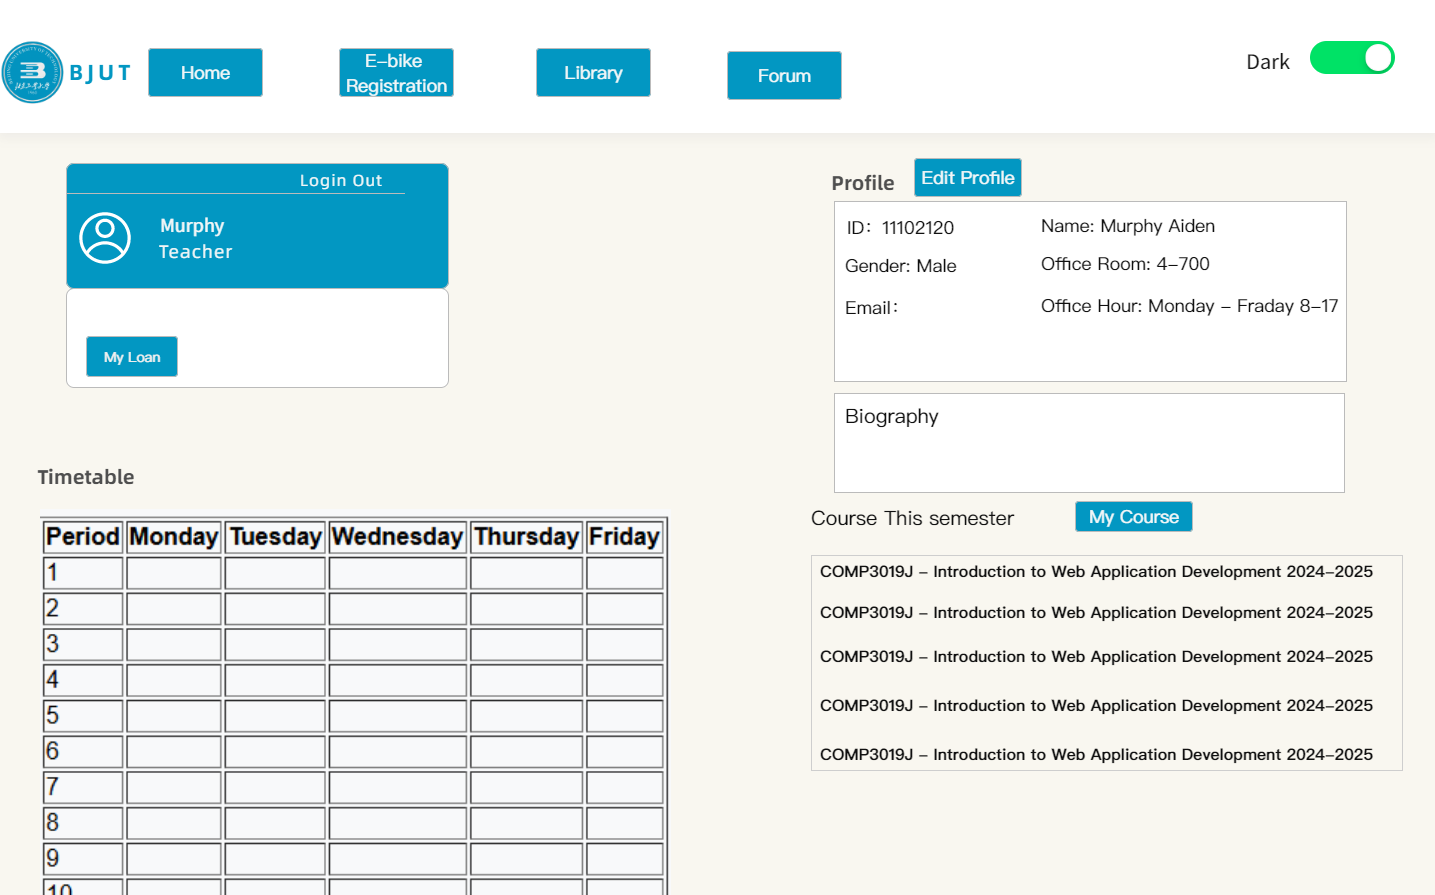
\includegraphics[width=\textwidth]{mockups/teacher/teacherdash.png}
    \caption{Teacher Dashboard}
    \label{fig:teacher_dashboard_page}
\end{figure}

\subsection{Mockups for library staff functions}

\begin{figure}[H]
    \centering
    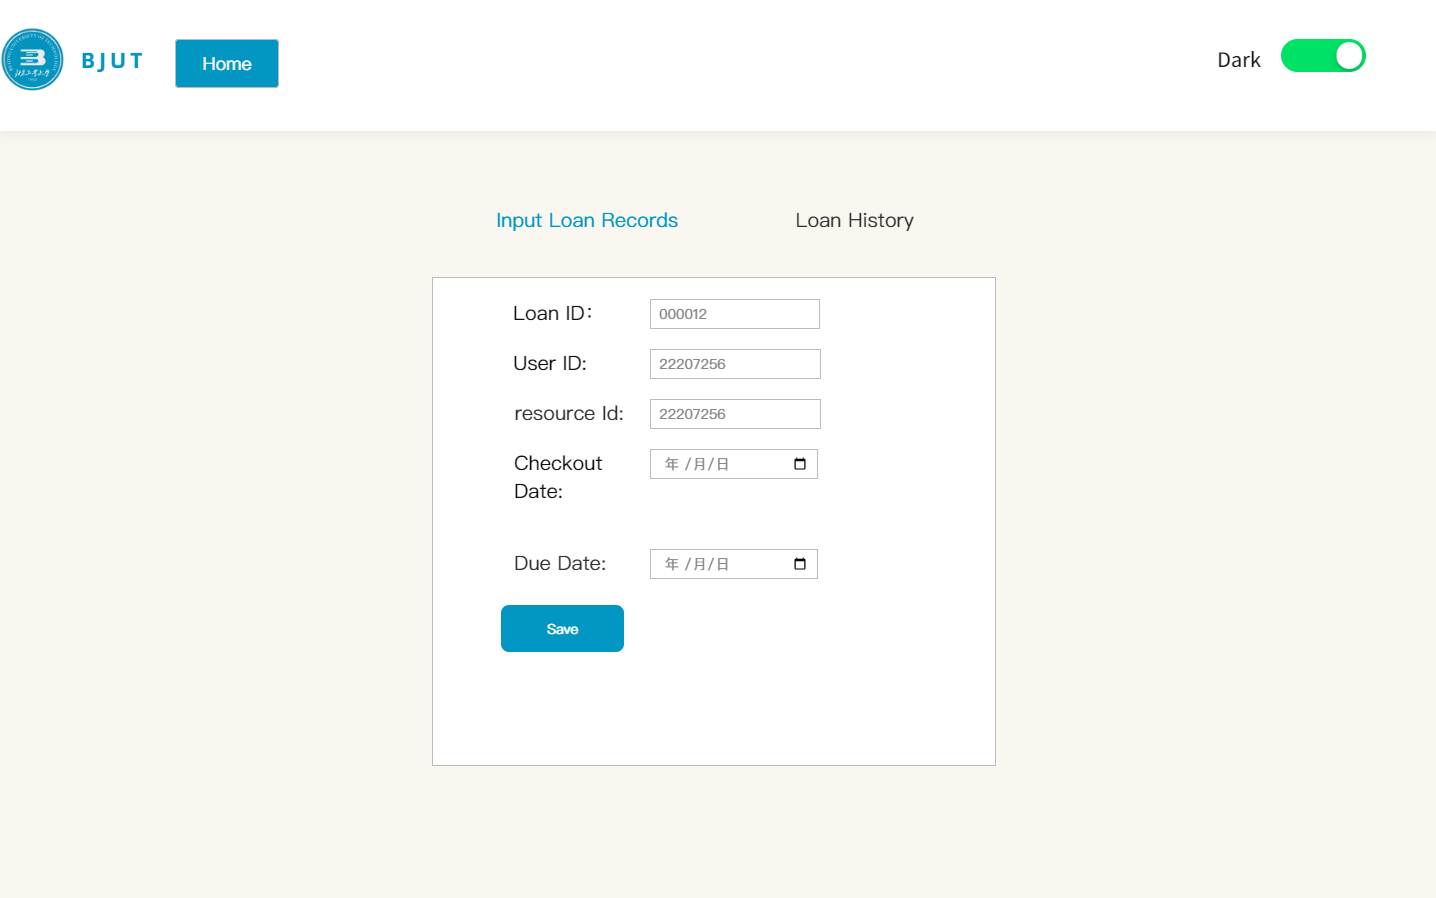
\includegraphics[width=\textwidth]{mockups/library/addloan.png}
    \caption{Add Loan Page}
    \label{fig:library_addloan_page}
\end{figure}

\begin{figure}[H]
    \centering
    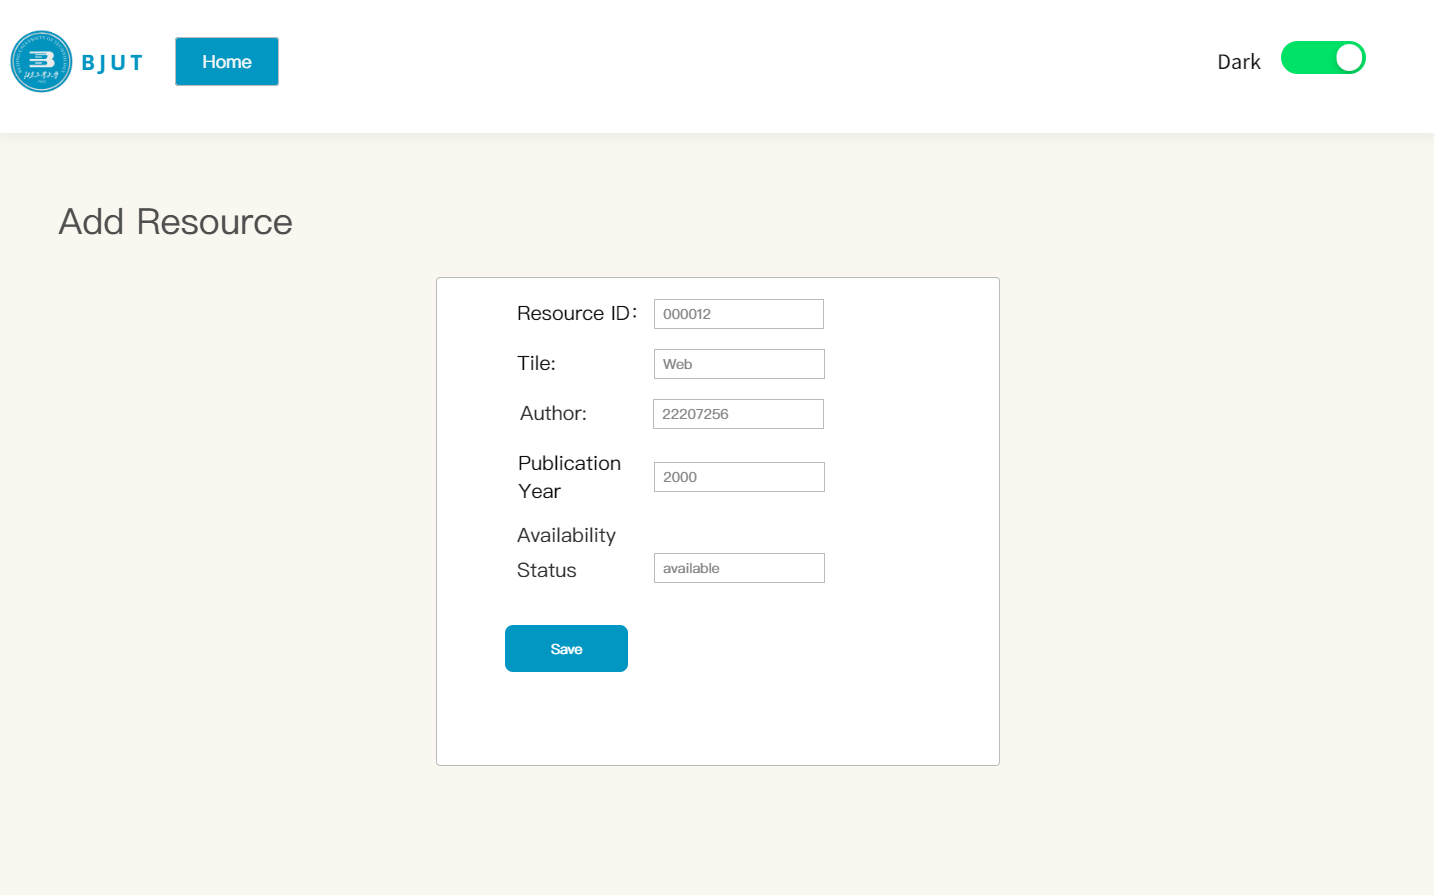
\includegraphics[width=\textwidth]{mockups/library/addresource.png}
    \caption{Add Resource Page}
    \label{fig:library_addresource_page}
\end{figure}

\begin{figure}[H]
    \centering
    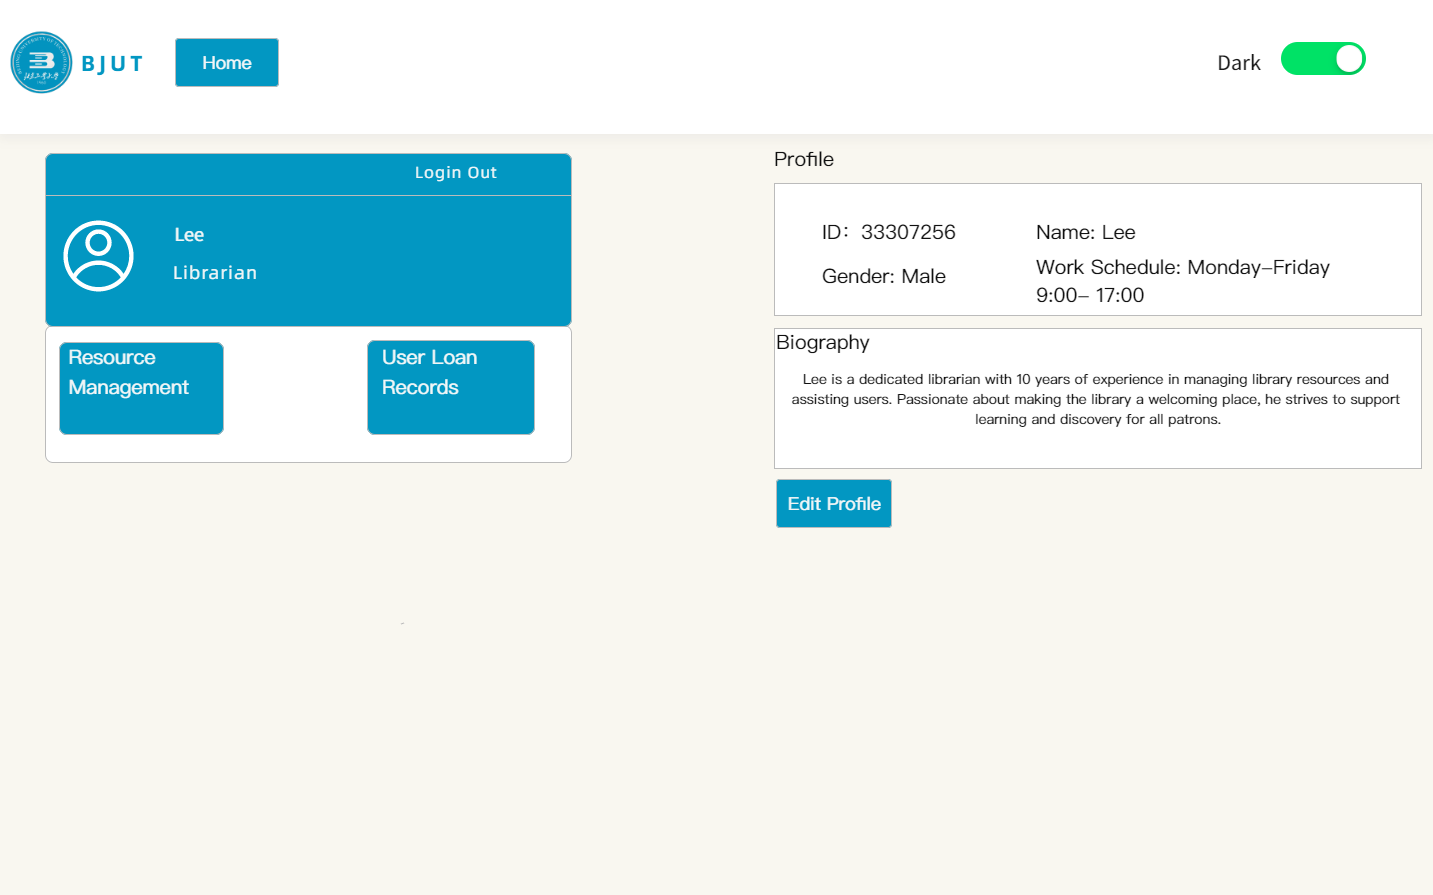
\includegraphics[width=\textwidth]{mockups/library/librarydash.png}
    \caption{Library Dashboard}
    \label{fig:library_dashboard_page}
\end{figure}

\begin{figure}[H]
    \centering
    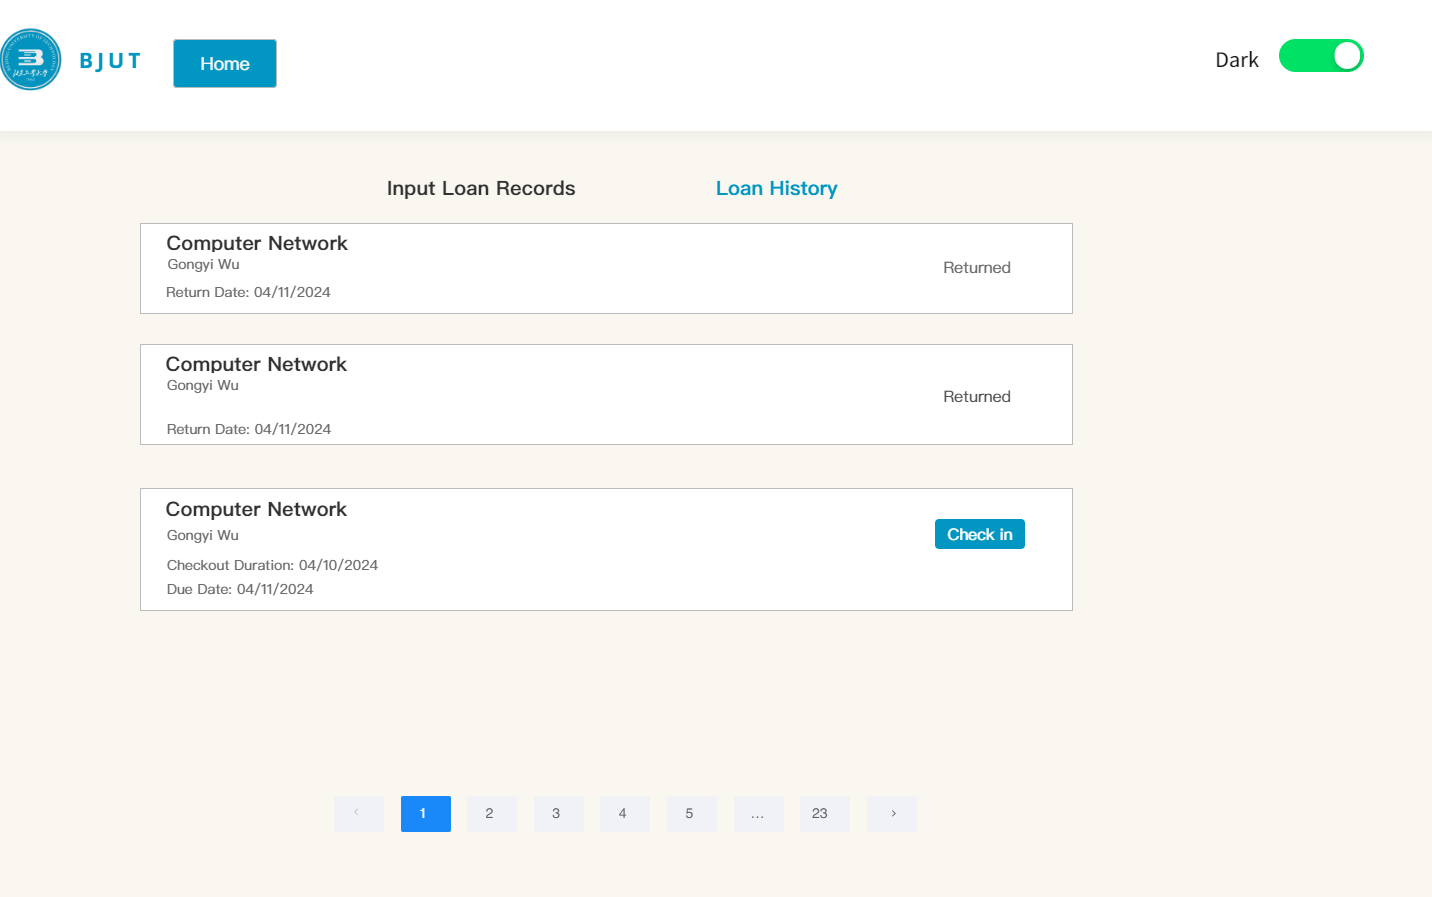
\includegraphics[width=\textwidth]{mockups/library/loanhistory.png}
    \caption{Loan History Page}
    \label{fig:library_loanhistory_page}
\end{figure}

\begin{figure}[H]
    \centering
    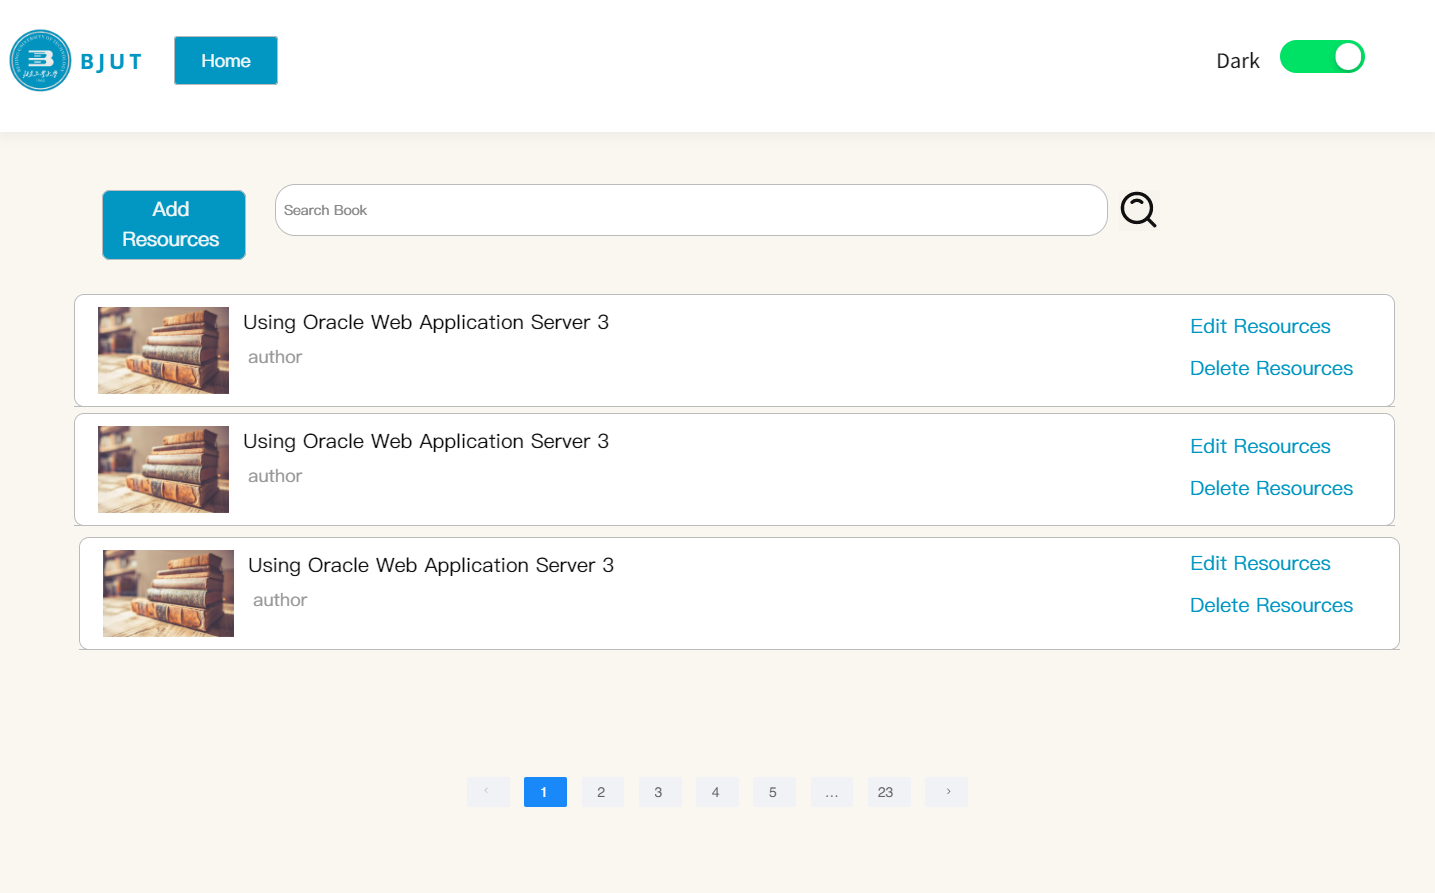
\includegraphics[width=\textwidth]{mockups/library/manageresource.png}
    \caption{Manage Resource Page}
    \label{fig:library_manageresource_page}
\end{figure}

\begin{figure}[H]
    \centering
    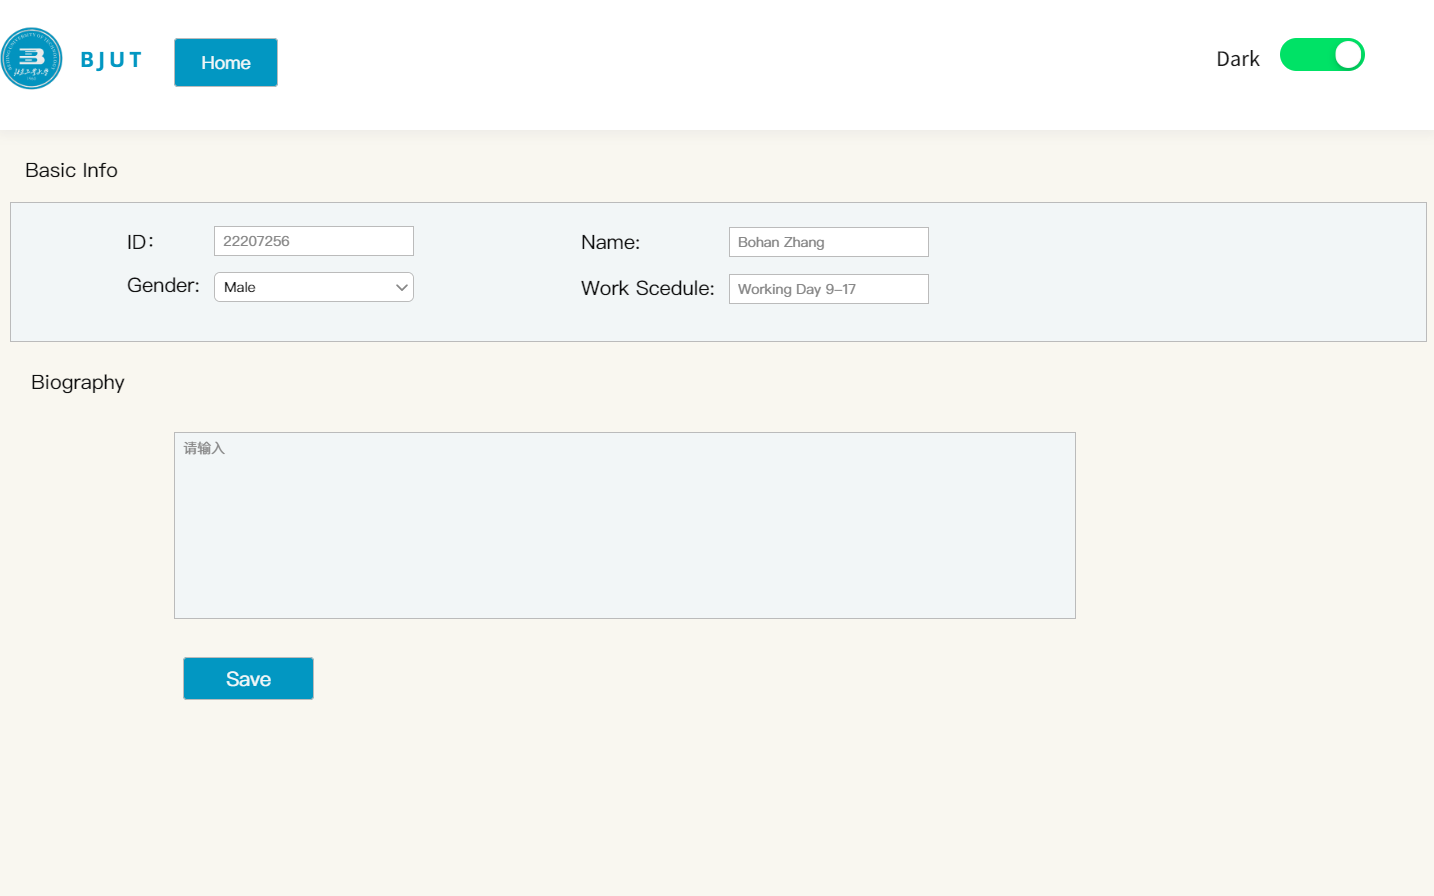
\includegraphics[width=\textwidth]{mockups/library/profile.png}
    \caption{Profile Page}
    \label{fig:library_profile_page}
\end{figure}

\subsection{Mockups for security personnel functions}

\begin{figure}[H]
    \centering
    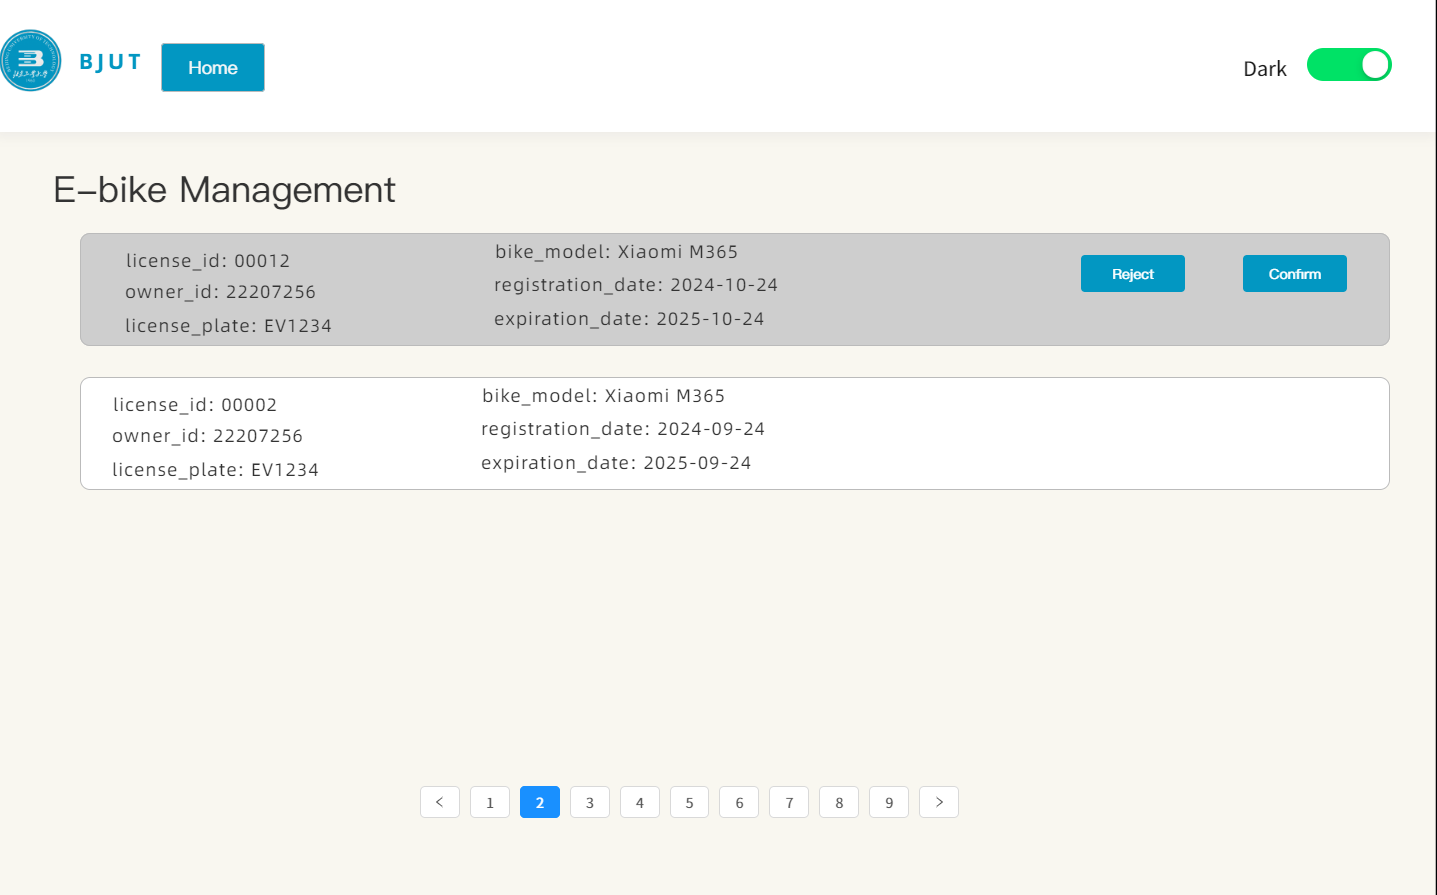
\includegraphics[width=\textwidth]{mockups/security/ebikemanage.png}
    \caption{E-bike Management Page}
    \label{fig:security_ebikemanage_page}
\end{figure}

\begin{figure}[H]
    \centering
    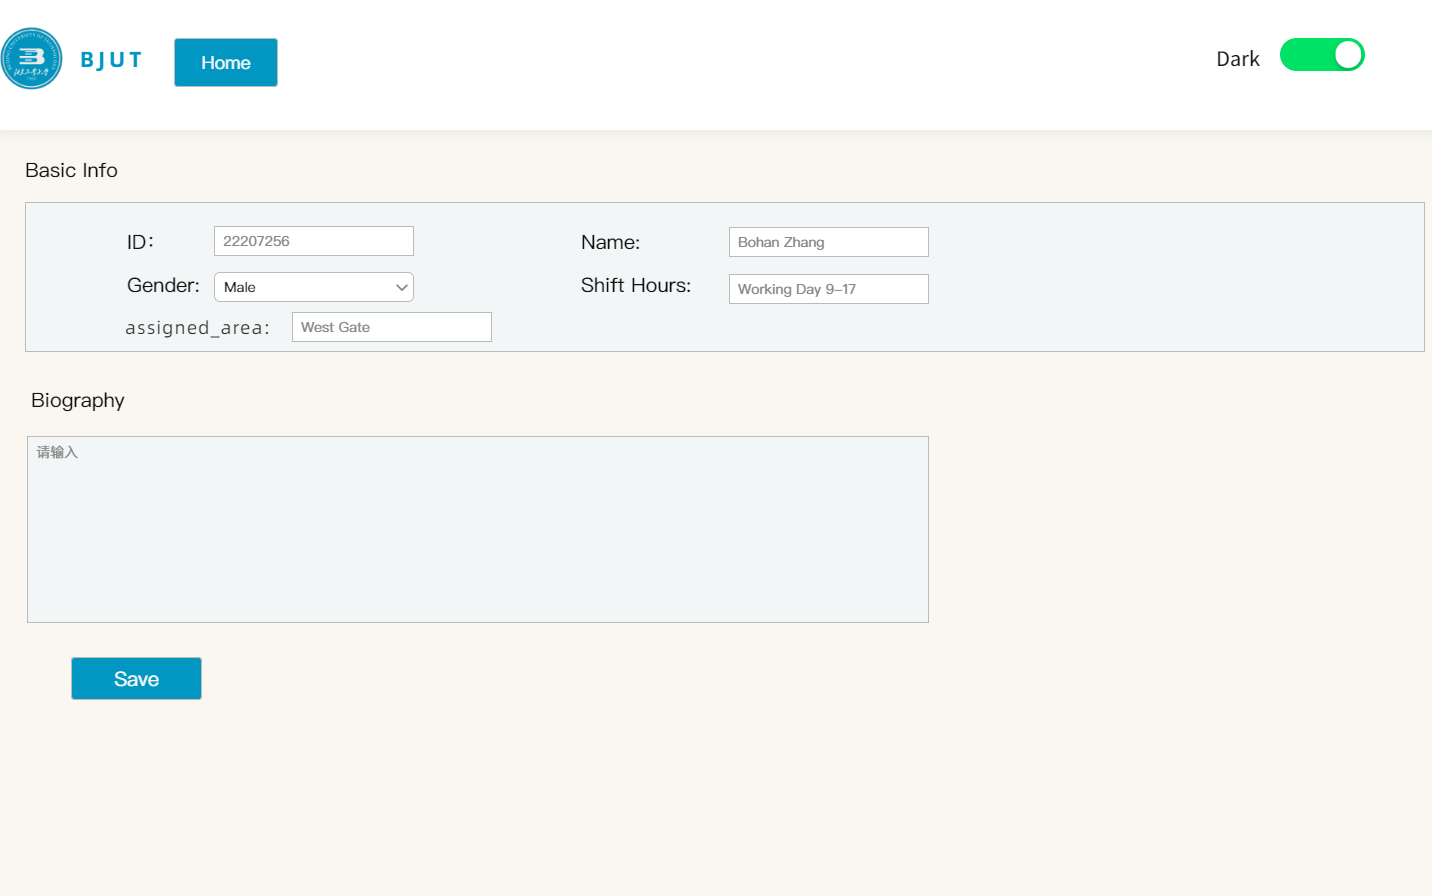
\includegraphics[width=\textwidth]{mockups/security/profile.png}
    \caption{Profile Page (Security Personnel)}
    \label{fig:security_profile_page}
\end{figure}

\begin{figure}[H]
    \centering
    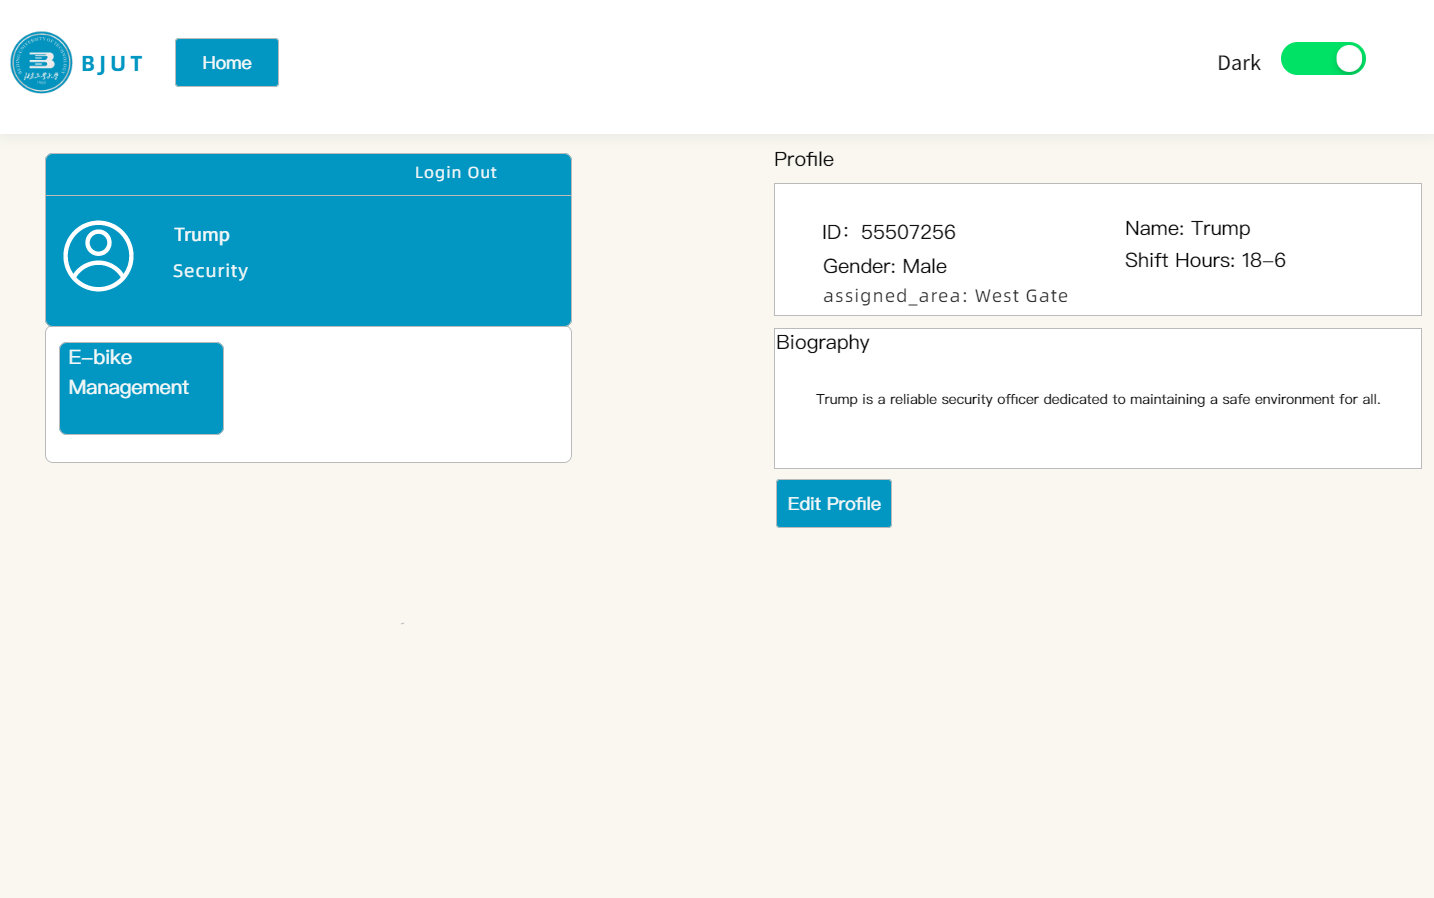
\includegraphics[width=\textwidth]{mockups/security/securitydash.png}
    \caption{Security Dashboard}
    \label{fig:security_dashboard_page}
\end{figure}

\subsection{Mockups for administrator functions}

\begin{figure}[H]
    \centering
    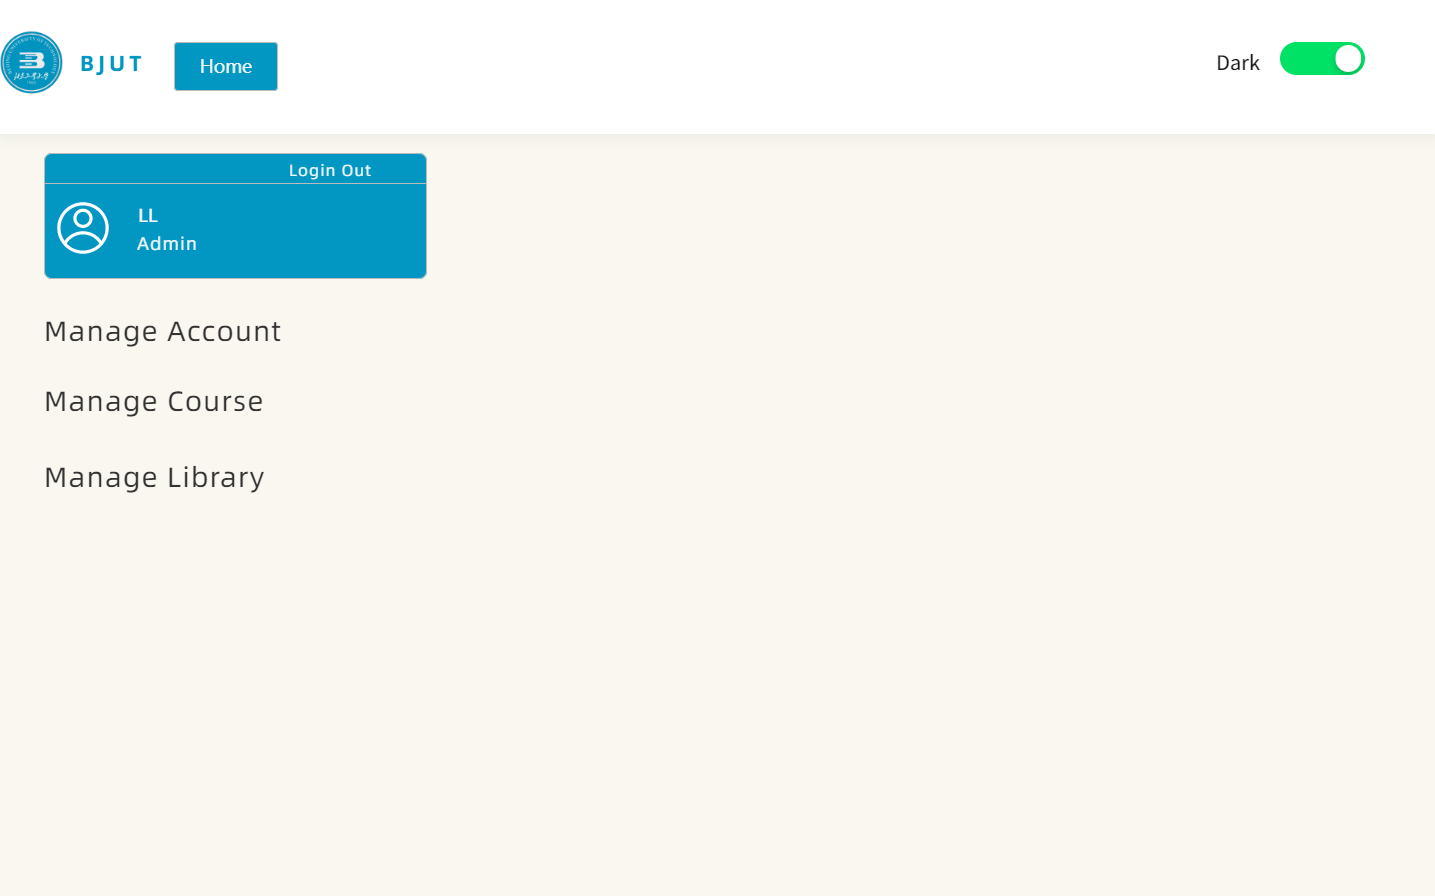
\includegraphics[width=\textwidth]{mockups/admin/admindash.png}
    \caption{Admin Dashboard}
    \label{fig:admin_dashboard_page}
\end{figure}

\begin{figure}[H]
    \centering
    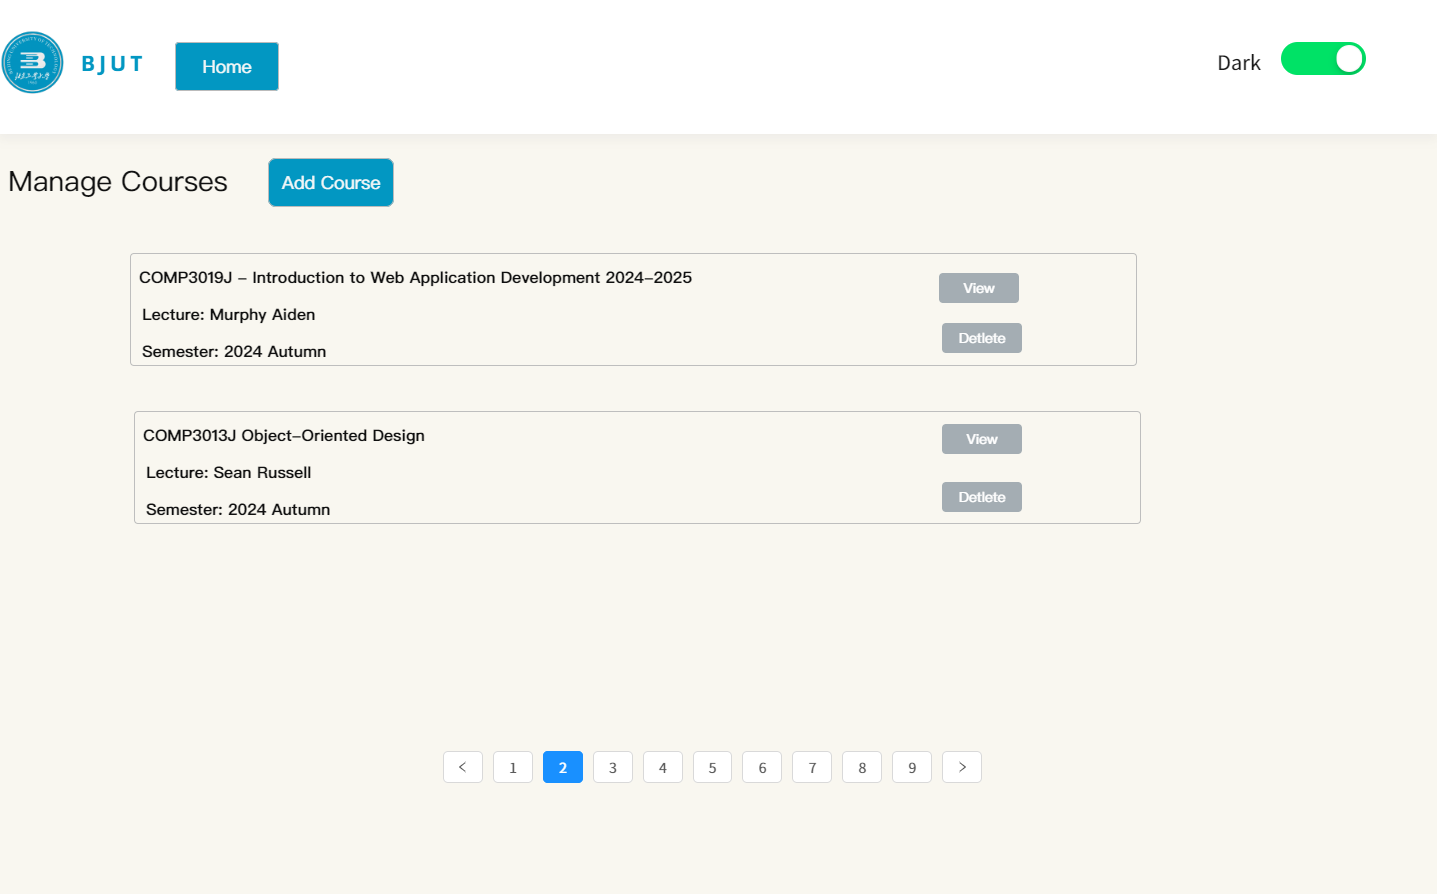
\includegraphics[width=\textwidth]{mockups/admin/courselist.png}
    \caption{Course List Page}
    \label{fig:admin_courselist_page}
\end{figure}

\begin{figure}[H]
    \centering
    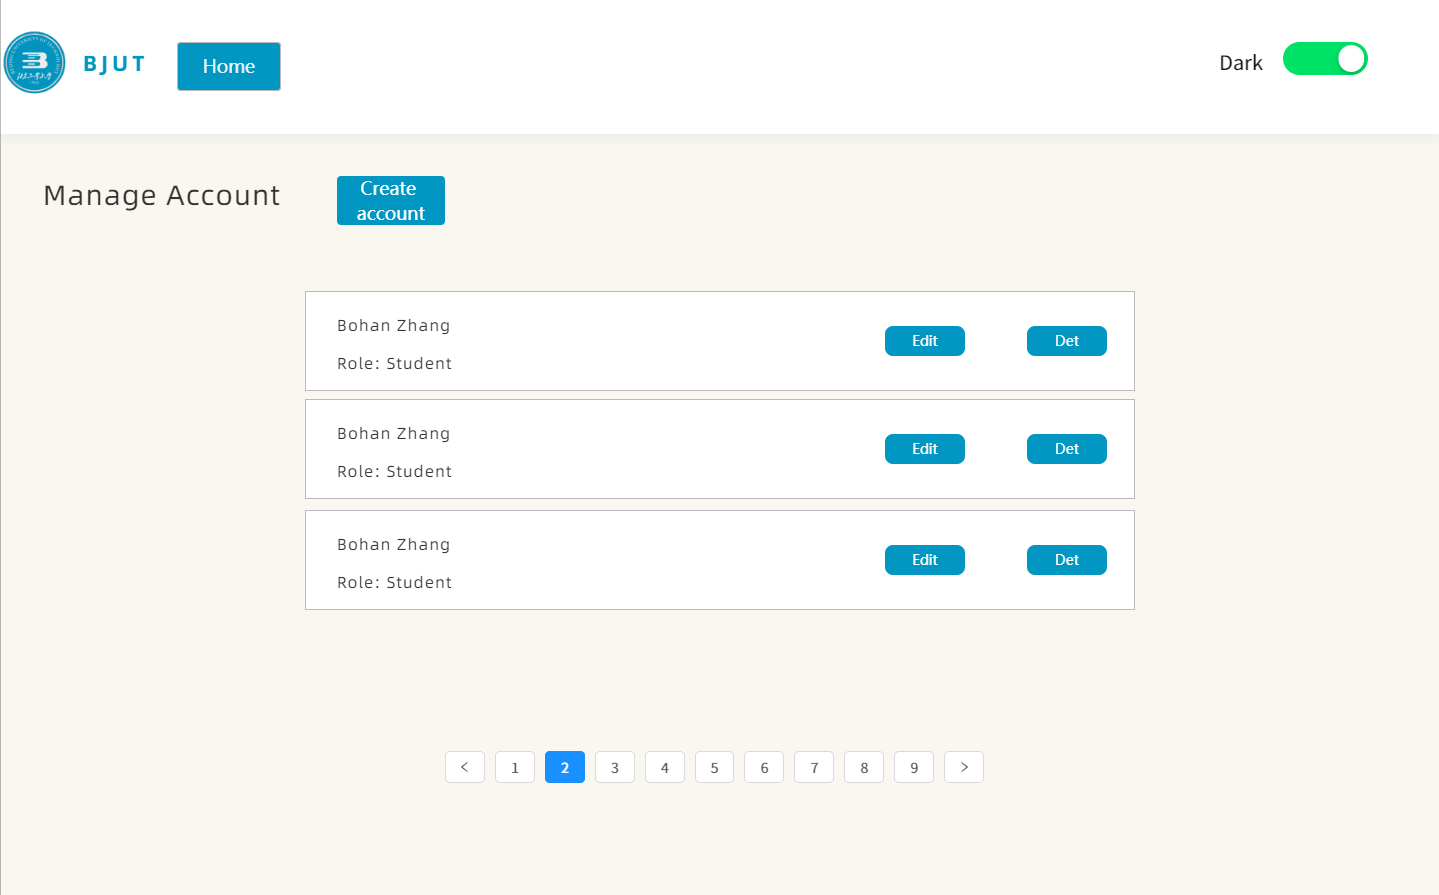
\includegraphics[width=\textwidth]{mockups/admin/useraccount.png}
    \caption{User Account Management Page}
    \label{fig:admin_useraccount_page}
\end{figure}

\subsection{Mockups for visitor functions}

\begin{figure}[H]
    \centering
    
\includegraphics[width=\textwidth]{mockups/visitor/contact.png}
    \caption{Contact Page}
    \label{fig:visitor_contact_page}
\end{figure}

\subsection{Color Schemes and Style Guidelines}
The interface uses a consistent blue and white color scheme aligned with the university’s branding. Interactive elements are highlighted with accent colors for clarity, and fonts are chosen for readability and accessibility.

\subsection{User Experience Considerations}
The design focuses on intuitive navigation, mobile responsiveness, and accessibility. Key elements like search, forum, and loan records are easy to locate, and feedback is provided for user actions to enhance usability.

\newpage

\section{Technical Details}

\subsection{File and Directory Structure}
The project is organized in the following file and directory structure:
\begin{itemize}
    \item \texttt{web-application/}: Root directory containing the main application, virtual environment, and project files.
    \begin{itemize}
        \item \texttt{app/}: Contains the main application logic and related files.
        \begin{itemize}
            \item \texttt{admin/}: Contains administrative functionality and management scripts.
            \item \texttt{api/}: Contains API endpoints and functions related to interactions between the web application and other services.
            \item \texttt{static/}: Stores static resources such as CSS files, JavaScript, and images.
            \item \texttt{templates/}: Contains the HTML files for rendering the front-end views.
            \item \texttt{\_\_init\_\_.py}: Initializes the application and its modules.
            \item \texttt{forms.py}: Contains the form classes used in the application, such as RegisterForm, LoginForm, TeacherProfileForm, StudentProfileForm, CreateCourseForm, and RegisterCourseForm.
            \item \texttt{models.py}: Defines the database models including User, Course, TeacherProfile, StudentProfile, and CourseRegistration.
            \item \texttt{routes.py}: Defines the routes (endpoints) for the web application, including login, logout, user profile, course creation, editing, and deletion.
        \end{itemize}
        \item \texttt{Project Document/}: Contains project documentation files, including design documents and technical reports.
        \item \texttt{tests/}: Directory for storing test cases for different modules.
        \begin{itemize}
            \item \texttt{test.py}: Contains unit and functional tests to validate the application features.
        \end{itemize}
        \item \texttt{.gitignore}: Specifies files and directories for Git to ignore.
        \item \texttt{config.py}: Contains the configuration settings for the application, including the MySQL database URI and secret keys.
        \item \texttt{README.md}: Readme file that provides an overview of the project, setup instructions, and other relevant information.
        \item \texttt{run.py}: The entry point for running the web application. This script starts the Flask server.
    \end{itemize}
\end{itemize}

\subsection{Code Components and Dependencies}
The application is built using Flask, a lightweight web framework for Python. The key components and their dependencies are:
\begin{itemize}
    \item \textbf{Flask Framework}: Provides the web framework for handling HTTP requests, routing, and rendering templates.
    \item \textbf{Flask-SQLAlchemy}: ORM for handling database interactions, providing seamless integration with MySQL for data persistence.
    \item \textbf{Flask-Login}: Manages user authentication and session management.
    \item \textbf{pymysql}: Used as the MySQL database driver for connecting to the remote database.
    \item \textbf{Werkzeug}: Provides password hashing and security utilities.
    \item \textbf{WTForms}: Provides form handling, validation, and CSRF protection.
    \item \textbf{Flask-Limiter}: Implements rate limiting to prevent abuse and ensure security.
\end{itemize}

\subsection{Database Interaction}
The application utilizes a remote MySQL database managed through SQLAlchemy, which acts as the Object Relational Mapper (ORM). The ORM abstracts the database operations into high-level Python objects, allowing the software framework to interact with the database seamlessly. CRUD (Create, Read, Update, Delete) operations are performed using model classes, which represent tables in the database.\\ \\ 
The database is remotely connected, with connection settings specified in the configuration file. The database connection is established during application initialization, ensuring a stable and secure interaction with the database throughout the application lifecycle. Below is the database host information:

\begin{table}[H]
    \centering
    \begin{tabular}{|c|c|c|}
        \hline
        \textbf{User} & \textbf{Database Host} & \textbf{Database Name} \\
        \hline
        root & \texttt{39.105.0.202:3306} & \texttt{WebApp} \\
        \hline
    \end{tabular}
    \caption{Database Host Information}
\end{table}

\subsection{Version Control and Repository Details}
The project uses Git for version control. The repository is hosted on GitLab, providing collaborative features such as pull requests, issue tracking, and version management. The main branch is used for stable releases, while development is done in separate feature branches. Commits are documented with clear messages, ensuring that changes are traceable, and the development workflow follows a feature-based branching model for effective collaboration.\\ \\
The repository can be accessed at: \url{https://csgitlab.ucd.ie/webApplication/web-application}
\newpage
\section{Conclusion}

\subsection{Summary of Features}
The university website project offers a range of functionalities to meet the needs of diverse user groups, including students, teachers, library staff, security personnel, administrative staff, and external visitors. Key features include:

\begin{itemize}
    \item \textbf{Student Dashboard}: Students can manage course registrations, check grades, view personal profiles, and register electric bikes.
    \item \textbf{Teacher Dashboard}: Teachers can manage courses, including creating, editing, and deleting courses, and handling student enrollments and grade entries.
    \item \textbf{Library Management}: Library staff can manage resources, process borrowing records, and monitor library inventory.
    \item \textbf{E-bike and Campus Security}: Security personnel can manage electric bike registrations and ensure compliance with campus regulations.
    \item \textbf{Administrative Controls}: Administrators can handle user management, system configurations, and ensure the proper functioning of the platform.
    \item \textbf{Forum and Customization Features}: Students and teachers can participate in forums for academic discussions, while all users can customize their interface preferences for an improved user experience.
\end{itemize}
The project successfully integrates personalized role-based dashboards, secure user authentication, and effective database management, offering a streamlined user experience for all stakeholders.

\subsection{Future Development Plans}
Future development plans for the university website project include:

\begin{itemize}
    \item \textbf{Enhanced User Experience}: Improving the user interface and experience by implementing more dynamic and responsive designs, optimizing navigation, and integrating user feedback mechanisms.
    \item \textbf{Advanced Role-Based Access Control}: Expanding role-based access control to facilitate more granular permission levels, including more administrative and library management features.
    \item \textbf{Automated Notifications and Alerts}: Adding features such as automated email notifications for course registration updates, grade availability, library due dates, and other user-specific events.
    \item \textbf{Analytics Dashboard}: Providing teachers and administrators with dashboards to monitor student engagement, analyze course registration trends, and track library resource usage.
    \item \textbf{Integration with External Systems}: Exploring integrations with learning management systems (LMS) and other external services to enhance the platform's capabilities.
    \item \textbf{Mobile Application Development}: Developing a mobile version of the platform to extend accessibility and usability on smartphones and tablets.
\end{itemize}
These future enhancements aim to improve functionality, provide deeper insights through analytics, and create a more connected and integrated educational environment. The ongoing development will continue to focus on user needs and adopting best practices to enhance performance and usability.


\end{document}